\documentclass[letterpaper,10pt]{memoir}
  \usepackage[T1]{fontenc}
  \usepackage[utf8]{inputenc}
  \usepackage[english,francais]{babel}
  \usepackage[autolanguage]{numprint}
  \usepackage{vgmath,vgsets,amsmath,icomma}
  \usepackage{pslatex}
  \usepackage[sc]{mathpazo}
  \usepackage[noae]{Sweave}
  \usepackage{graphicx,color}
  \usepackage{longtable,lscape} % table de loi F
  \usepackage[absolute]{textpos}
  \usepackage{answers}
  \usepackage[alwaysadjust,defblank]{paralist}

  %%% Hyperliens
  \usepackage{hyperref}
  \definecolor{link}{rgb}{0,0,0.3}
  \hypersetup{
    pdftex,
    colorlinks,%
    citecolor=link,%
    filecolor=link,%
    linkcolor=link,%
    urlcolor=link}

 %%% Page titre
  \title{\HUGE
    \fontseries{ub}\selectfont Séries chronologiques \\[0.5\baselineskip]
    \huge\fontseries{m}\selectfont Exercices et solutions}
  \author{\LARGE François Pelletier \\[3mm]
    \large École d'actuariat \\ Université Laval \\[6mm]
  }
  \date{Première édition - Automne 2013}
  \newcommand{\ISBN}{}

  %%% Sous-figures
  \newsubfloat{figure}

  %%% Style des entêtes de chapitres
  \chapterstyle{hangnum}

  %%% Styles des entêtes et pieds de page
  \setlength{\marginparsep}{7mm}
  \setlength{\marginparwidth}{13mm}
  \setlength{\headwidth}{\textwidth}
  \addtolength{\headwidth}{\marginparsep}
  \addtolength{\headwidth}{\marginparwidth}

  %%% Style de la bibliographie
  \bibliographystyle{francais}

  %%% Options de babel
  \frenchbsetup{CompactItemize=false,%
    ThinSpaceInFrenchNumbers=true}
  \addto\captionsfrench{\def\tablename{{\scshape Tab.}}}
  \addto\captionsfrench{\def\figurename{{\scshape Fig.}}}

  %%% Associations entre les environnements et les fichiers
  \Newassociation{sol}{solution}{solutions}
  \Newassociation{rep}{reponse}{reponses}

  %%% Environnement pour les exercices
  \newcounter{exercice}[chapter]
  \newenvironment{exercice}{%
     \begin{list}{\bfseries \arabic{chapter}.\arabic{exercice}}{%
         \refstepcounter{exercice}
         \settowidth{\labelwidth}{\bfseries \arabic{chapter}.\arabic{exercice}}
         \setlength{\leftmargin}{\labelwidth}
         \addtolength{\leftmargin}{\labelsep}
         \setdefaultenum{a)}{i)}{}{}}\item}
     {\end{list}}

  %%% Environnement pour les réponses
  \renewenvironment{reponse}[1]{%
    \begin{list}{\bfseries #1}{%
        \settowidth{\labelwidth}{#1}
        \setlength{\leftmargin}{\labelwidth}
        \addtolength{\leftmargin}{\labelsep}
        \setdefaultenum{a)}{i)}{}{}}\item}
    {\end{list}}
  \renewcommand{\reponseparams}{{\thechapter.\theexercice}}

  %%% Environnement pour les solutions
  \renewenvironment{solution}[1]{%
    \begin{list}{\bfseries #1}{%
        \settowidth{\labelwidth}{#1}
        \setlength{\leftmargin}{\labelwidth}
        \addtolength{\leftmargin}{\labelsep}
        \setdefaultenum{a)}{i)}{}{}}\item}
    {\end{list}}
  \renewcommand{\solutionparams}{{\thechapter.\theexercice}}

  %%% Nouvelles commandes
  \newcommand{\cov}[1]{\mathrm{Cov} ( #1 )}
  \renewcommand{\Cov}[1]{\mathrm{Cov}\! \left( #1 \right)}
  \newcommand{\prob}[1]{\mathrm{Pr} [ #1 ]}
  \newcommand{\Prob}[1]{\mathrm{Pr}\! \left[ #1 \right]}
  \newcommand{\MSE}{\mathrm{MSE}}

  %%% Environnements pour le code S: police plus petite
  \RecustomVerbatimEnvironment{Sinput}{Verbatim}{fontshape=sl,fontsize=\small}
  \RecustomVerbatimEnvironment{Soutput}{Verbatim}{fontsize=\small}
  \RecustomVerbatimEnvironment{Scode}{Verbatim}{fontsize=\small}

  %%% Un petit peu d'aide pour la césure
  \hyphenation{con-fiance}
  \hyphenation{con-train-te}

\DeclareMathOperator{\sgn}{sgn}

\begin{document}

\frontmatter

\pagestyle{empty}
%%% Police de caractère pour la page titre
\renewcommand{\sfdefault}{hls}

%%% Marge de gauche (1/3 de la page)
\newlength{\gauche}
\addtolength{\gauche}{72mm}
\addtolength{\gauche}{-\spinemargin}

%%% Épaisseur de la bande sur la page titre
\newlength{\ruleheight}
\setlength{\ruleheight}{7.75mm}

%%% Définition de la bande
\definecolor{gray}{gray}{0.4}
\textblockorigin{0mm}{279mm}
\newcommand{\banderecto}{%
  \begin{textblock*}{71.5mm}[0,1](0mm,-46.5mm)
    \textblockcolor{black} \rule{0mm}{\ruleheight}
  \end{textblock*}
  \begin{textblock*}{144mm}[0,1](72mm,-46.5mm)
    \textblockcolor{gray} \rule{0mm}{\ruleheight}
  \end{textblock*}}
\newcommand{\bandeverso}{%
  \begin{textblock*}{144mm}[0,1](0mm,-46.5mm)
    \textblockcolor{gray} \rule{0mm}{\ruleheight}
  \end{textblock*}
  \begin{textblock*}{71.5mm}[0,1](144.5mm,-46.5mm)
    \textblockcolor{black} \rule{0mm}{\ruleheight}
  \end{textblock*}}

%%% Titre
\begin{adjustwidth*}{\gauche}{-15mm}
  \sffamily\fontseries{ub}\selectfont
  \raggedright
  \vspace*{2cm}
  \thetitle
\end{adjustwidth*}

%%% Affichage de la bande
\banderecto
\cleardoublepage

%%% Page de garde
\begin{adjustwidth*}{\gauche}{-15mm}
  \sffamily\fontseries{ub}\selectfont
  \raggedright
  \vspace*{2cm}
  \thetitle \\
  \bfseries
  \vspace*{3cm}
  \theauthor
  \vspace*{\fill}
  \thedate
\end{adjustwidth*}

\clearpage

%%% Page de notices
\begingroup
\calccentering{\unitlength}
\begin{adjustwidth*}{\unitlength}{-\unitlength}
  \small
  \setlength{\parindent}{0pt}
  \setlength{\parskip}{\baselineskip}

  {\textcopyright} 2013 François Pelletier \\


  
\includegraphics[height=7mm,keepaspectratio=true]{by}\;%
  
\includegraphics[height=7mm,keepaspectratio=true]{sa} \\
  Cette création est mise à disposition selon le contrat
  Paternité-Partage des conditions initiales à l'identique 2.5 Canada
  disponible en ligne
  \url{http://creativecommons.org/licenses/by-sa/2.5/ca/} ou par
  courrier postal à Creative Commons, 171 Second Street, Suite 300,
  San Francisco, California 94105, USA.

  \textbf{Historique de publication}
  \vspace{-\baselineskip}
  \begin{tabbing}
    Décembre 2013:\quad\= Première édition
  \end{tabbing}

  \textbf{Code source} \\
  Le code source {\LaTeX} de ce document est disponible à l'adresse
  \begin{quote}
    \url{https://github.com/franc00018/ACT-2010-Exercices}
  \end{quote}
  ou en communiquant directement avec les auteurs.

  \vspace{1cm}

  % ISBN \ISBN \\
  % Dépôt légal -- Bibliothèque et Archives nationales du Québec, 2014 \\
  % Dépôt légal -- Bibliothèque et Archives Canada, 2014
\end{adjustwidth*}
\endgroup

%%% Retour à la police normale
\renewcommand{\sfdefault}{phv}

\clearpage

%%% Local Variables:
%%% mode: latex
%%% TeX-master: "exercices_series_chrono"
%%% coding: utf-8-unix
%%% End:


\pagestyle{companion}

\cleardoublepage
\tableofcontents

\mainmatter

\documentclass[11pt,english,francais]{article}
\usepackage{scrtime}
\usepackage{natbib} 
\usepackage{tikz} 
\usepackage{multirow}
\usepackage[utf8]{inputenc}
\usepackage{amsmath} 
\usepackage{amsfonts} 
\usepackage{amsthm} 
\usepackage{thmtools}
\usepackage{hyperref}
\usepackage{cleveref}
\usepackage[hypcap]{caption}
\usepackage[off]{auto-pst-pdf}
\usepackage[scale=2]{ccicons}
\usepackage{tabularx}
\DeclareMathOperator{\sgn}{sgn}

\begin{document}


\section{Méthodes de lissage et saisonnalité}
\label{sec:serie-dexercices-1}

\subsection{Noël s'en vient ! (Informatique)}
\label{sec:exercice-1-1}

On considère les taux d'inflation sur 12 mois disponibles dans le
fichier \url{cg130823a001-fra.csv}. On représente cette série chronologique
par la variable aléatoire $Y_t$. L'an passé, les Canadiens ont dépensé
en moyenne $674\$$ en cadeaux au mois de décembre 2012. Notre objectif
est de prévoir quel sera le montant dépensé pour l'achat de cadeaux en
décembre 2013.

\begin{enumerate}
\item Tracez un graphique de la série chronologique $Y_t$ à l'aide
  d'un logiciel statistique. Êtes vous en mesure de déceler
  visuellement la présence d'une tendance et/ou d'une saisonnalité ?

\item Utilisez l'opérateur différentiel $\nabla_{12}$ afin d'éliminer
  la saisonnalité annuelle de la série chronologique $Y_t$ et obtenir
  la série $Z_t$. Tracez à nouveau un graphique avec les données
  obtenues. Remarquez-vous toujours la présence de saisonnalité ?
  Tracez le graphique de la composante de saisonnalité $s_t$.

\item Maintenant, nous voulons déceler s'il y a présence d'une
  tendance dans les données. En utilisant la méthode de la moyenne
  mobile avec $q=1$ et $q=5$, du lissage exponentiel double avec
  $\alpha=5\%$ et de la régression linéaire simple, estimer la
  tendance $\hat{m}_t$. Faire le graphique superposé des 5 tendances.

\item En utilisant le résultat de la régression linéaire précédente,
  prévoir la valeur non saisonnalisée en décembre 2013. En évaluant la
  moyenne des différences entre la série $Y_t$ et la valeur de la
  régression pour les mois de décembre des années précédente, on peut
  estimer la valeur $\hat{s}_{12}$. Ajouter cette valeur au résultat
  obtenu pour obtenir une estimation du taux d'inflation en décembre
  2013.

\item En applicant ce taux d'inflation à la donnée du problème,
  prédire le montant dépensé pour l'achat de cadeaux en décembre 2013.
\end{enumerate}

\subsection{Incendies (Calculatrice)}

On a estimé la tendance d’un ensemble de données d’incendie pour une
année. Cependant, suite à un problème informatique, certaines données
sont manquantes. Identifiez ces données.\\

\begin{tabular}{|l|l|l|l|}
  \hline
  \multicolumn{1}{|l|}{Mois} & \multicolumn{1}{l|}{Incendies} & \multicolumn{1}{l|}{Moyenne Mobile} &  \\ \hline
  1 & 4 & \multicolumn{1}{l|}{-} &  \\ \hline
  2 & 3 & \multicolumn{1}{l|}{-} &  \\ \hline
  3 & \multicolumn{1}{l|}{a} & 4,8 &  \\ \hline
  4 & \multicolumn{1}{l|}{b} & 4,8 &  \\ \hline
  5 & 2 & 5,4 &  \\ \hline
  6 & 4 & 5,2 &  \\ \hline
  7 & 6 & 3,6 &  \\ \hline
  8 & \multicolumn{1}{l|}{c} & 3,6 &  \\ \hline
  9 & \multicolumn{1}{l|}{0} & 4,4 &  \\ \hline
  10 & 2 & 3,8 &  \\ \hline
  11 & 8 & \multicolumn{1}{l|}{-} &  \\ \hline
  12 & 3 & \multicolumn{1}{l|}{-} &  \\ \hline
\end{tabular}

\subsection{Option de vente (Calculatrice)}

Nous sommes le 28 juin 2013, à l'heure de la fermeture des marchés
financiers. Vous possédez un titre de la compagnie BlackBerry dont la
valeur est de $S_0 = 10.46$. Un analyste vous suggère d'acheter une
option de vente européenne d'échéance de 84 jours ($t=84/365$) avec un prix d'exercice
équivalant à la valeur d'un contrat à terme de même échéance afin de
couvrir le risque de baisse de la valeur de ce titre. On considère des
rendements sur une période de 28 jours et un taux sans risque composé
continument de $r=1.75\%$.  En utilisant les logarithmes des valeurs
historique à la fermeture du titre disponibles dans le fichier
\url{blackberry.csv}, ainsi que la méthode de différenciation,
évaluez les rendements mensuels du titre, qui correspondent aux
résidus de ce processus différentié. Ensuite, en évaluant la moyenne
et l'écart-type de cette composante, il est possible d'estimer la
tendance linéaire $\mu$ et la volatilité $\sigma$ mensuelles de la
série des rendements. En supposant que le prix peut prendre deux
valeurs après 3 mois, soit $S_0u = S_0 e^{3(\mu+\sigma/(2\sqrt{3}))}$
et $S_0d = S_0 e^{3(\mu-\sigma/(2\sqrt{3}))}$, évaluez le prix de
l'option de vente en utilisant la probabilité neutre au risque d'une
hausse $p^{*} = \frac{e^{rt}-d}{u-d}$ et évaluez le profit que vous
effectuerez en exercant l'option de vente le 20 septembre 2013,
considérant que vous empruntez au taux $r+2\%$ pour acheter l'option.

\subsection{Lissage exponentiel I (Calculatrice)}

On considère un ensemble de 10 observations:
\[
\mathcal{A}=\left\{1.2,1.5,1.4,2.1,1.8,1.9,2.2,2.4,2.0,1.9 \right\}
\]

En utilisant une méthode de lissage exponentiel avec $\alpha=0.4$ et
$\alpha=0.7$, déterminez laquelle des méthodes produit la moins grande
erreur quadratique moyenne (MSE).

\subsection{Lissage exponentiel II (Informatique)}

En utilisant les données du problème précédent, déterminez, à l'aide
d'un algorithme informatique, la valeur de $\alpha$ qui minimise
l'erreur quadratique moyenne (MSE).

\subsection{Bank of America (calculatrice)}

On considère les 20 observations de la valeur ajustée à la fermeture (valeur qui tient compte des dividendes) du titre de la Bank of America pour chaque lundi entre le 20 mai 2013 et le 30 septembre 2013. Ces données se trouvent dans le fichier \url{BoA.csv}.

\begin{enumerate}
\item En utilisant le test du corrélogramme avec un seuil de tolérance de $\alpha = 10\%$, déterminez s'il s'agit d'une série stationnaire.

\item En utilisant le test du changement de direction, déterminez s'il s'agit d'une série stationnaire.

\item En utilisant le test de Portmanteau avec un seuil de tolérance de $\alpha = 10\%$, déterminez s'il s'agit d'une série stationnaire.

\item Est-ce que ces tests sont équivalents ? Commentez.

\item En utilisant la différenciation et le logarithme des données, évaluez la série des rendements hebdomadaires.

\item En utilisant le même principe que pour la moyenne mobile, évaluez la variance mobile de la série précédente avec $q=2$. Que remarquez-vous ? Peut-on affirmer que c'est une série stationnaire à l'aide du test de Portmanteau avec  un seuil de tolérance de $\alpha = 10\%$?
\end{enumerate}

\subsection{Variance d'une série non-stationnaire (théorique)}
\label{sec:variance-dune-serie}

Une série présentant une racine unitaire se présente sous la forme $Y_t = Y_{t-1}+\epsilon_t$. Quelle est la différence entre la variance du $5^e$ terme et du $7^e$ terme de cette série si $\epsilon_t \sim N(0, 0.1t^2)$?

\clearpage


\includegraphics[height=7mm,keepaspectratio=true]{by-sa}\\%
Cette création est mise à disposition selon le contrat
\href{http://creativecommons.org/licenses/by-sa/2.5/ca/deed.fr}{%
  Paternité-Partage à l'identique 2.5 Canada} de Creative Commons
disponible à l'adresse \\
http://creativecommons.org/licenses/by-sa/2.5/ca/deed.fr \\

En vertu de ce contrat, vous êtes libre de :

\begin{itemize}
\item \textbf{partager} --- reproduire, distribuer et communiquer
  l'{\oe}uvre;
\item \textbf{remixer} --- adapter l'{\oe}uvre;
\item utiliser cette {\oe}uvre à des fins commerciales.
\end{itemize}

Selon les conditions suivantes:\\

  \begin{tabularx}{\linewidth}{@{}lX@{}}
    \raisebox{-9mm}[0mm][13mm]{%
      
\includegraphics[height=11mm,keepaspectratio=true]{by}} &
    \textbf{Attribution} --- Vous devez attribuer l'{\oe}uvre de la
    manière indiquée par l'auteur de l'{\oe}uvre ou le titulaire des
    droits (mais pas d'une manière qui suggérerait qu'ils vous
    soutiennent ou
    approuvent votre utilisation de l'{\oe}uvre). \\
    \raisebox{-9mm}{
\includegraphics[height=11mm,keepaspectratio=true]{sa}}
    & \textbf{Partage à l'identique} --- Si vous modifiez, transformez
    ou adaptez cette {\oe}uvre, vous n'avez le droit de distribuer
    votre création que sous une licence identique ou similaire à
    celle-ci.
  \end{tabularx}

\end{document}
%%% Local Variables: 
%%% mode: latex
%%% TeX-master: t
%%% End: 

\chapter{Modèles classiques pour séries chronologiques}
\label{chap:modeles-classiques}

\Opensolutionfile{reponses}[reponses-modeles-classiques]
\Opensolutionfile{solutions}[solutions-modeles-classiques]

\begin{Filesave}{reponses}
\bigskip
\section*{Réponses}

\end{Filesave}

\begin{Filesave}{solutions}
\section*{Chapitre \ref{chap:modeles-classiques}}
\addcontentsline{toc}{section}{Chapitre \protect\ref{chap:modeles-classiques}}

\end{Filesave}


\begin{exercice}
  Pour avoir la stationnarité, il faut que les racines du polynôme caractéristique soient inférieures à 1 en valeur absolue. Démontrez que pour le modèle AR(2), la stationnarité est possible si et seulement si les trois conditions suivantes sont réunies:
\begin{align*}
  \phi_1 + \phi_2 &< 1 \\
  \phi_2 - \phi_1 &< 1 \\
  |\phi_2| &< 1
\end{align*}
\begin{sol}
  On obtient les racines de l'équation caractéristique en utilisant la formule quadratique habituelle

\begin{align*}
\frac{\phi_1\pm\sqrt{\phi_1^2+4\phi_2}}{-2\phi_2}
\end{align*}

On considère les inverses des deux racines, $A_1$ et $A_2$.

\begin{align*}
A_1 &= \frac{2\phi_2}{-\phi_1-\sqrt{\phi_1^2+4\phi_2}} \\
&= \frac{2\phi_2}{-\phi_1-\sqrt{\phi_1^2+4\phi_2}} \left[\frac{-\phi_1+\sqrt{\phi_1^2+4\phi_2}}{-\phi_1+\sqrt{\phi_1^2+4\phi_2}} \right] \\
&= \frac{2\phi_2(-\phi_1+\sqrt{\phi_1^2+4\phi_2})}{\phi_1^2-(\phi_1^2+4\phi_2)}\\
&= \frac{\phi_1-\sqrt{\phi_1^2+4\phi_2}}{2}\\
A_2 &= \frac{\phi_1+\sqrt{\phi_1^2+4\phi_2}}{2}
\end{align*}

Il y a 2 situations possibles: soit les racines sont réelles ($\phi_1^2+4\phi_2>0$) ou elles sont complexes ($\phi_1^2+4\phi_2<0$).
\begin{itemize}
\item \textbf{Racines réelles:}
Comme les racines doivent être plus grandes que 1, alors nécessairement leurs inverses $|A_1|<1$ et $|A_2|<1$. Nous avons donc:
\begin{align*}
-1 &< \frac{\phi_1-\sqrt{\phi_1^2+4\phi_2}}{2} <  \frac{\phi_1+\sqrt{\phi_1^2+4\phi_2}}{2} < 1 \\
\Leftrightarrow -2 &< \phi_1-\sqrt{\phi_1^2+4\phi_2} < \phi_1+\sqrt{\phi_1^2+4\phi_2} < 2
\end{align*}
En observant la première inégalité, on a:
\begin{align*}
-2 < \phi_1-\sqrt{\phi_1^2+4\phi_2}
&\Leftrightarrow \sqrt{\phi_1^2+4\phi_2}<\phi_1+2 \\
&\Leftrightarrow \phi_1^2+4\phi_2 < \phi_1^2+4\phi_1+4 \\
&\Leftrightarrow \phi_2 < \phi_1 + 1 \\
&\Leftrightarrow \phi_2 - \phi_1 < 1
\end{align*}
Ce qui correspond à la seconde condition. En considérant la seconde inégalité, on obtient, de la même façon, la première inégalité:
\begin{align*}
\phi_1+\sqrt{\phi_1^2+4\phi_2} &< 2 \\
&\Leftrightarrow \phi_1 + \phi_2 < 1
\end{align*}
Ces deux conditions réunies avec un discriminant positif forment la région de stationnarité pour des racines réelles.

\item \textbf{Racines complexes:}  
On considère la situation où $\phi_1^2+4\phi_2<0$. Ici, on aura des conjugués complexes et $|A_1| = |A_2| <1$ seulement si $|A_1|^2<1$.
\begin{align*}
|A_1|^2 &=\frac{\phi_1^2+(-\phi_1^2-4\phi_2}{4}=-\phi^2 \\
&\Leftrightarrow \phi_2>-1 \\
&\Leftrightarrow |\phi_2|<1
\end{align*}
Ce résultat réuni avec un discriminant négatif forment la région de stationnarité pour des racines complexes.
\end{itemize}
\end{sol}
\end{exercice}




\begin{exercice}
  \begin{enumerate}
\item 
Un polynôme d'ordre $k$ en t est intégré d'ordre $k$ puisque
\begin{align*}
  (1-B)^k(a_0+a_1t+a_2t^2+\ldots+a_kt^k) &= k!a_k 
\end{align*}

Démontrez cette affirmation.
\item 

Démontrez que si $x_t$ est stationnaire, alors $(1-B)x_t$ est aussi stationnaire.
\end{enumerate}

\begin{sol}
\begin{enumerate}

\item On obtient ce résultat par récurrence. Par exemple, pour $k=2$, on a :

\begin{align*}
(1-B)^2 (a_0+a_1t+a_2t^2) &= (1-B) ((a_0+a_1t+a_2t^2)\\ &\quad- (a_0+a_1(t-1)+a_2(t-1)^2)) \\
&= (1-B) (a_1+a_2(2t+1)) \\
&= (a_1+a_2(2t+1)) - (a_1+a_2(2(t-1)+1)) \\
&= 2a_2
\end{align*}

En général, on obtient:

\begin{align*}
(1-B)^k (a_0+a_1t+a_2t^2+\ldots+a_kt^k) &= (1-B)^{k-1} ((a_0+a_1t+a_2t^2+\ldots+a_kt^k)\\ &\quad- (a_0+a_1(t-1)+a_2(t-1)^2+\ldots+a_k(t-1)^k)) \\
&= (1-B)^{k-1} (a_1 + 2a_2t+\ldots+a_k(t^k-(t-1)^k))
\end{align*}

On remarque qu'à chaque itération, le premier terme de la série disparait. Ainsi, après $k$ itérations, il ne restera que le terme en $a_k$ avec son coefficient, qui correspont à $k!$. On obtient ainsi la solution générale.

\item Une série est dite stationnaire lorsque chaque terme est un terme d'erreur dont la distribution est constante au fil du temps. Ainsi, la distribution de la différence de deux termes consécutifs de la série sera aussi constante au fil du temps. Par exemple:
\begin{align*}
\epsilon_t \sim N(0,\sigma^2)  \\
\epsilon_t - \epsilon_{t-1} \sim N(0,2\sigma^2) \\
\end{align*}

\end{enumerate}
\end{sol}
\end{exercice}


\begin{exercice}
  \begin{enumerate}
\item 
Démontrez algébriquement qu'un processus AR(1) est équivalent à un processus MA($\infty$).

\item 
Démontrez algébriquement qu'un processus MA(1) est équivalent à un processus AR($\infty$).
\end{enumerate}
\begin{sol}
  \begin{enumerate}
\item Un processus AR(1) est défini par $y_t = \phi_1y_{t-1} + \epsilon_t$. En développant le terme $y_{t-1}$, on obtient $y_t = \phi_1^2y_{t-2}+\phi_1\epsilon_{t-1}+\epsilon_t$. De manière récursive, on obtient $y_t = \phi_1^{t}\epsilon_0 + \phi_1^{t-1}\epsilon_1 + \ldots + \phi_1\epsilon_{t-1} + \epsilon_t$. ainsi, en faisant tendre $t\to\infty$, on obtient une représentation MA($\infty$).

\item Un processus MA(1) est défini par $y_t = \epsilon_t - \theta_1\epsilon_{t-1}$. On cherche à substituer le terme $\epsilon_{t-1}$. On développe le terme précédent de la série: $y_{t-1} = \epsilon_{t-1} - \theta_1\epsilon_{t-2}$ et on substitue dans la première expression pour obtenir $y_t = \epsilon_t - \theta_1y_{t-1} - \theta_1^2\epsilon_{t-2}$. De manière récursive, on obtient $y_t = -\theta_1^ty_0-\theta_1^{t-1}y_1-\ldots-\theta_1y_{t-1}+\epsilon_{t}$. Lorsque $t\to\infty$, on obtient une représentation AR($\infty$).
\end{enumerate}
\end{sol}
\end{exercice}


\begin{exercice}
  On considère les 10 nombres aléatoires suivants, issus d'une distribution normale centrée réduite:

\begin{verbatim}
 [1] -1.21  0.28  1.08 -2.35  0.43  0.51 -0.57 -0.55 -0.56 -0.89
\end{verbatim}

Construisez la série autorégressive d'ordre 1 avec coefficient: 
\begin{enumerate}
\item $\phi = -0.5$
\item $\phi = 0.5$
\end{enumerate}

Quelle différence observez-vous entre la série avec une corrélation négative et la série avec une corrélation positive ?
\begin{sol}
  On utilise la formule $y_t = \phi_1y_{t-1} + \epsilon_t$.

\begin{center}
\begin{tabular}{|r|r|r|}
\hline
\multicolumn{1}{|l|}{} & \multicolumn{ 2}{c|}{$\phi$} \\ \hline
\multicolumn{1}{|l|}{$N(0,1)$} & -0,5 & 0,5 \\ \hline
-1,21 & -1,2100 & -1,2100 \\ \hline
0,28 & 0,8850 & -0,3250 \\ \hline
1,08 & 0,6375 & 0,9175 \\ \hline
-2,35 & -2,6688 & -1,8913 \\ \hline
0,43 & 1,7644 & -0,5156 \\ \hline
0,51 & -0,3722 & 0,2522 \\ \hline
-0,57 & -0,3839 & -0,4439 \\ \hline
-0,55 & -0,3580 & -0,7720 \\ \hline
-0,56 & -0,3810 & -0,9460 \\ \hline
-0,89 & -0,6995 & -1,3630 \\ \hline
\end{tabular}
\end{center}

Les séries avec une corrélation négative ont tendance à aller dans la direction contraire des termes précédents alors que celles avec une corrélation positive ont tendance à aller dans la même direction que les termes précédents.

Le tableur \url{constructionserieAR.ods} contient les calculs effectués.
\end{sol}
\end{exercice}

\begin{exercice}
  On considère deux processus MA(2), un où $\theta_1 = \theta_2 = \frac{1}{4}$, et un autre où $\theta_1=-1$ et $\theta_2 = 4$. Démontrez que ces processus ont la même fonction d'autocorrélation.
  \begin{sol}
    Il suffit de calculer la fonction d'autorégression pour chaque processus MA(2).
Ensuite, on peut évaluer la fonction d'autocorrélation et comparer le résultat obtenu.

\begin{enumerate}
\item Premier processus avec:
\begin{align*}
\theta_1 = \theta_2 = \frac{1}{4}
\end{align*}
Fonction d'autocovariance
\begin{align*}
\phi_0^{(1)} &= V[Y_t] \\
&= V[e_t]+\frac{1}{16}V[e_{t-1}]+\frac{1}{16}V[e_{t-2}] \\
&= (1+\frac{1}{8})\theta^2_e \\
&= \frac{9}{8} \sigma^2_e \\
\end{align*}
\begin{align*}
\phi_1^{(1)} &= Cov(Y_t,Y_{t-1}) \\
&= Cov(e_t - \frac{1}{4}e_{t-1} - \frac{1}{4}e_{t-2}, e_{t-1} - \frac{1}{4}e_{t-2} - \frac{1}{4}e_{t-3} )\\
&= Cov(-\frac{1}{4}e_{t-1},e_{t-1}) + Cov(-\frac{1}{4}e_{t-2},-\frac{1}{4}e_{t-2}) \\
&= (-\frac{1}{4}+(-\frac{1}{4})(-\frac{1}{4})) \sigma^2_e \\
&= -\frac{3}{16} \sigma^2_e \\
\end{align*}
\begin{align*}
\phi_2^{(1)} &= Cov(Y_t,Y_{t-2}) \\
&= Cov(e_t - \frac{1}{4}e_{t-1} - \frac{1}{4}e_{t-2}, e_{t-2} - \frac{1}{4}e_{t-3} - \frac{1}{4}e_{t-4} )\\
&= Cov(-\frac{1}{4}e_{t-2},e_{t-2}) \\
&= -\frac{1}{4} \sigma^2_e \\
\end{align*}
\begin{align*}
\phi_k^{(1)} &= 0, \qquad \forall k \geq 3
\end{align*}
Fonction d'autocorrélation
\begin{align*}
\rho_1^{(1)} &= \frac{\phi_1^{(1)}}{\phi_0^{(1)}} \\
&= \frac{\frac{-3}{16}\sigma^2_e}{\frac{9}{8}\sigma^2_e} \\
&= \frac{-1}{6} \\
\end{align*}
\begin{align*}
\rho_2^{(1)} &= \frac{\phi_2^{(1)}}{\phi_0^{(1)}} \\
&= \frac{\frac{-1}{4}\sigma^2_e}{\frac{9}{8}\sigma^2_e} \\
&= \frac{-2}{9} \\
\end{align*}
\item Second processus avec:
\begin{align*}
\theta_1 = -1 \quad \theta_2 = 4
\end{align*}
Fonction d'autocovariance
\begin{align*}
\phi_0^{(2)} &= V[Y_t] \\
&= V[e_t]+V[e_{t-1}]+16V[e_{t-2}] \\
&= 18 \sigma^2_e
\end{align*}
\begin{align*}
\phi_1^{(2)} &= Cov(Y_t,Y_{t-1}) \\
&= Cov(e_t + e_{t-1} - 4e_{t-2}, e_{t-1} + e_{t-2} - 4e_{t-3}) \\
&= Cov(e_{t-1},e_{t-1}) + Cov(-4e_{t-2},e_{t-2}) \\
&= (1 + (-1)(4))\sigma^2_e \\
&= -3\sigma^2_e \\
\end{align*}
\begin{align*}
\phi_2^{(2)} &= Cov(Y_t,Y_{t-2}) \\
&= Cov(e_t + e_{t-1} - 4e_{t-2}, e_{t-2} + e_{t-3} - 4e_{t-4} )\\
&= Cov(- 4e_{t-2},e_{t-2}) \\
&= -4\sigma^2_e \\
\end{align*}
Fonction d'autocorrélation
\begin{align*}
\rho_1^{(2)} &= \frac{\phi_1^{(2)}}{\phi_0^{(2)}} \\
&= \frac{-3\sigma^2_e}{18\sigma^2_e} \\
&= \frac{-1}{6} \\
\end{align*}
\begin{align*}
\rho_2^{(2)} &= \frac{\phi_2^{(2)}}{\phi_0^{(2)}} \\
&= \frac{-4\sigma^2_e}{18\sigma^2_e} \\
&= \frac{-2}{9} \\
\end{align*}
\end{enumerate}

On remarque clairement que $\rho_1^{(1)} = \rho_1^{(2)}$ et $\rho_2^{(1)} = \rho_2^{(2)}$. 
La fonction d'autocovariance vaut toujours 1 pour $\rho_1$ et vaut 0 ailleurs.
  \end{sol}
\end{exercice}


\begin{exercice}
  \begin{enumerate}
\item En utilisant les équations de Yule-Walker, dérivez un estimateur des moments pour les paramètres $\phi_1$ et $\phi_1$ d'un processus AR(2). \\

\item Estimez les paramètres du processus AR(2) à partir de la série suivante:
\begin{verbatim}
 [1]  1.1617660  0.6981185  0.1693004 -0.6457205  1.4217278  1.3701445
 [7] -1.6369769 -0.4596686 -0.2933815 -1.0995973
\end{verbatim}
\end{enumerate}
\begin{sol}
  \begin{enumerate}
\item 
Les deux équations de Yule-Walker pour le modèle AR(2) sont les suivantes:
\begin{align*}
\rho_1 = \phi_1 + \rho_1 \phi_2 \\
\rho_2 = \rho_1\phi_1 + \phi_2
\end{align*}

En utilisant l'estimateur de la fonction d'autocovariance $\hat{\rho}$, on obtient alors:

\begin{align*}
\hat{\phi_1} = \frac{\hat{\rho_1}(1-\hat{\rho_2})}{1-\hat{\rho_1}^2} \\
\hat{\phi_2} = \frac{\hat{\rho_2} - \hat{\rho_1}^2}{1-\hat{\rho_1}^2}
\end{align*}


\item

\begin{Schunk}
\begin{Sinput}
> set.seed(123)
> (serie <- arima.sim(n = 10, list(ar = c(0.5,-0.25))))
\end{Sinput}
\begin{Soutput}
Time Series:
Start = 1 
End = 10 
Frequency = 1 
 [1]  1.1617660  0.6981185  0.1693004 -0.6457205
 [5]  1.4217278  1.3701445 -1.6369769 -0.4596686
 [9] -0.2933815 -1.0995973
\end{Soutput}
\begin{Sinput}
> acf.serie <- acf(serie,type="correlation",plot=FALSE)$acf[2:3]
> phi1 <- acf.serie[1]*(1-acf.serie[2]) / (1-acf.serie[1]^2)
> phi2 <- (acf.serie[2] - acf.serie[1]^2) / (1-acf.serie[1]^2)
\end{Sinput}
\end{Schunk}

On obtient $\hat{\rho_1} = 0.07455$ et $\hat{\rho_2} = -0.28041$. 
Ce qui nous donne les paramètres du modèle AR(2) suivants:
$\hat{\phi_1} = 0.09599$ et 
$\hat{\phi_2} = -0.28757$.
\end{enumerate}
\end{sol}
\end{exercice}


\begin{exercice}
  \begin{enumerate}
\item Démontrez que le terme d'erreur $\epsilon_t$ d'un processus ARMA(2,1) peut être exprimé sous la forme suivante, où $\mu$ est une constante et $\phi_1, \phi_2, \theta$ sont les paramètres du modèle. On considère que la série est stationnaire.
\begin{align*}
  \epsilon_t = \sum_{i=0}^{\infty} \theta^i \left(y_{t-i} - \mu - \phi_1 y_{t-i-1} - \phi_2 y_{t-i-2} \right)
\end{align*}

\item De plus, démontrez qu'à partir de cette forme du terme d'erreur, on peut obtenir la représentation AR($\infty$) du processus ARMA(2,1).
\end{enumerate}
\begin{sol}
  \begin{enumerate}
\item
  On représente le processus ARMA(2,1) sous la forme suivante:
  \begin{align*}
    y_t = \mu + \phi_1 y_{t-1} + \phi_2 y_{t-2} + \epsilon_t - \theta\epsilon_{t-1}
  \end{align*}
  
  En utilisant l'opérateur de rétrodécalage $B$, on peut exprimer cette équation sous la forme suivante:
  \begin{align*}
    (1-\theta B)\epsilon_t = y_t - \mu - \phi_1 y_{t-1} - \phi_2 y_{t-2}
  \end{align*}
  
  On divise ensuite de chaque côté par $(1-\theta B)$, pour obtenir:
  \begin{align*}
    \epsilon_t = \frac{1}{(1-\theta B)} \left(y_t - \mu - \phi_1 y_{t-1} - \phi_2 y_{t-2}\right)
  \end{align*}
  
  L'hypothèse de stationnarité nous permet de poser que $| \theta | < 1$, ce qui nous permet d'utiliser la série géométrique définie comme suit:
  \begin{align*}
    \frac{1}{1-\theta B} = \sum_{i=0}^{\infty} \theta^i B^i
  \end{align*}
  
  On obtient donc que 
  \begin{align*}
    \epsilon_t = \sum_{i=0}^{\infty} \theta^i B^i \left(y_t - \mu - \phi_1 y_{t-1} - \phi_2 y_{t-2}\right)
  \end{align*}
  
  En appliquant l'opérateur de rétrodécalage à la parenthèse, on obtient la solution:
  \begin{align*}
    \epsilon_t = \sum_{i=0}^{\infty} \theta^i \left(y_{t-i} - \mu - \phi_1 y_{t-i-1} - \phi_2 y_{t-i-2} \right)
  \end{align*}

\item
  
  On exprime l'équation précédente en fonction de $y_t$:
  \begin{align*}
    y_t &= \phi_1 y_{t-1} + \phi_2 y_{t-2} - \sum_{i=1}^{\infty} \theta^i \left(y_{t-i} - \phi_1 y_{t-i-1} - \phi_2 y_{t-i-2} \right) + \epsilon_t + \frac{\mu}{1-\theta} \\
    &= \phi_1 y_{t-1} + \phi_2 y_{t-2} - \left[\theta\left(y_{t-1}-\phi_1 y_{t-2} - \phi_2 y_{t-3} \right) + \sum_{i=2}^{\infty} \theta^i \left(y_{t-i} - \phi_1 y_{t-i-1} - \phi_2 y_{t-i-2} \right)\right] + \epsilon_t + \frac{\mu}{1-\theta}  \\
    &= (\phi_1 - \theta) y_{t-1} - \sum_{i=2}^{\infty} \left(\theta_i+\phi_1\theta^{i-1} - \phi_2\theta_{i-2}\right) y_{t-i} + \epsilon_t + \frac{\mu}{1-\theta}
  \end{align*}
  Ce qui correspont à la forme autorégressive AR($\infty$) suivante:
  \begin{align*}
    y_t = c + \sum_{i=1}^{\infty} \pi_i y_{t-i} + \epsilon_t
  \end{align*}
  Avec les paramètres
  \begin{align*}
    c &= \frac{\mu}{1-\theta} \\
    \pi_1 &= (\phi_1 - \theta) \\
    \pi_i &= -\left(\theta_i+\phi_1\theta^{i-1} - \phi_2\theta_{i-2}\right),\quad i=2,3,\ldots
  \end{align*}
\end{enumerate}
\end{sol}
\end{exercice}

\begin{exercice}
  On considère l'équation en différence suivante:
\begin{align*}
  y_t = 1.5 y_{t-1} - 0.5 y_{t-2} + \epsilon_t
\end{align*}
\begin{enumerate}
\item À quel modèle correspond cette équation ?
\item Trouvez les racines de l'équation homogène.
\item Démontrez que les racines de l'équation $1-1.5B+0.5B^2$ sont la réciproque des valeurs trouvées à la question précédente.
\item Est-ce que cette série est stationnaire ?
\item On suppose que l'on connaît les deux premiers termes de la série $y_0$ et $y_1$. Trouvez la solution générale pour $y_t$ en fonction de la séquence des valeurs de $\epsilon_t$.
\item Identifiez la forme de la fonction de prédiction pour $y_{T+s}$, sachant les valeurs de $y_{T-1}$ et $y_T$.
\item Évaluez $E[y_t]$, $E[y_{t+1}]$, $Var[y_t]$, $Var[y_{t+1}]$ et $Cov[y_{t},y_{t+1}]$.
\item Donnez l'expression d'un intervalle de confiance à 95\% pour la valeur de $y_{t+1}$ 
\end{enumerate}
\begin{sol}
  \begin{enumerate}
\item C'est un modèle AR(2) de paramètres $\phi_1=1.5$ et $\phi_2=-0.5$.
\item L'équation caractéristique prend la forme suivante:
  \begin{align*}
    y_t - 1.5 y_{t-1} + 0.5y_{t-2} = 0
  \end{align*}
  
  On pose la solution générale $y_t=A\alpha^t$:
  \begin{align*}
    A\alpha^t - 1.5 A\alpha^{t-1} + 0.5A\alpha^{t-2} = 0
  \end{align*}
  
  On divise ensuite par $A\alpha^{t-2}$:
  \begin{align*}
    0 &= \alpha^2 - 1.5 \alpha + 0.5\\
    \alpha &= \frac{1.5 \pm \sqrt{1.5^2-4*1*0.5}}{2} \\
    &= \left\{0.5 ; 1 \right\}
  \end{align*}

\item
  \begin{align*}
    1 - 1.5B + 0.5B^2 &= 0 \\
    (1-B)(1-0.5B) &= 0
  \end{align*}
  Ce qui nous donne:
  \begin{align*}
    B &= \left\{ 1;2 \right\} \\
    B^{-1} &= \left\{ 1;0.5 \right\}
  \end{align*}

\item Nous n'avons pas la stationnarité, car $\alpha$ n'est pas à l'intérieur du cercle unité

\item
  \begin{align*}
    y_2 &= 1.5 y_1 - 0.5y_0 + \epsilon_2 \\
    y_3 &= 1.5 y_2 - 0.5y_1 + \epsilon_3 \\
    &= \epsilon_3 + 1.5 \epsilon_2 + 1.75y_1 - 0.75 y_0 \\
    y_4 &= 1.5 y_3 - 0.5y_2 + \epsilon_4 \\
    &= \epsilon_4 + 1.5 \epsilon_3 + 1.75 \epsilon_2 + 1.875 y_1 - 0.875 y_0
  \end{align*}
  
  On peut observer un motif répétifif, que l'on représente sous la forme
  \begin{align*}
    y_t &= \sum_{i=0}^{t-2} \alpha_i\epsilon_{t-i} + \alpha_{t-1}y_1 + \alpha_t y_0 \\
  \end{align*}
  où 
  \begin{align*}
    \alpha_0 &= 1\\ 
    \alpha_1 &= 1.5\\
    \alpha_t &= 1-\alpha_{t-1}
    \alpha_i &= 1.5 \alpha_{i-1} - 0.5 \alpha_{i-2}
  \end{align*}
\item 
  \begin{align*}
    y_s &= \sum_{i=0}^{s-2} \alpha_i\epsilon_{s-i} + \alpha_{s-1}y_1 + \alpha_s y_0 \\
    y_{t+s} &= \sum_{i=0}^{s-2} \alpha_i\epsilon_{t+s-i} + \alpha_{s-1}y_{t+1} + \alpha_s y_t \\
    E_{t+1}\left[y_{t+s}\right] &= \alpha_{s-1} y_{t+1} + \alpha_s y_t
  \end{align*}

\item
  \begin{align*}
    E\left[y_t\right] &= \alpha_{t-1} y_1 + \alpha_t y_0 \\
    E\left[y_{t+1}\right] &= \alpha_{t} y_1 + \alpha_{t+1} y_0 \\
    Var\left[y_t\right] &= \left[1+\alpha_1^2 + \alpha_2^2 + \ldots + \alpha_{t-2}^2\right]\sigma^2 \\
    Var\left[y_{t+1}\right] &= Var\left[y_t\right] + \alpha_{t-1}^2 \sigma^2 \\
    Cov\left[y_{t},y_{t+1}\right] &= \left[\alpha_0\alpha_1 + \alpha_1\alpha_2 + \ldots + \alpha_{t-3}\alpha_{t-2}\right] \sigma^2
  \end{align*}
\item
  \begin{align*}
    \alpha_{t} y_1 + \alpha_{t+1} y_0 \pm 1.96 * \sigma \sqrt{1+\alpha_1^2 + \alpha_2^2 + \ldots + \alpha_{t-2}^2+\alpha_{t-1}^2}
  \end{align*}
\end{enumerate}
\end{sol}
\end{exercice}


\begin{exercice}
  Soit les deux processus suivants:
\begin{align*}
Y_t &= V_t + \alpha V_{t-1} \\
Z_t &= \delta_t
\end{align*}

On ajoute que $V_t$ et $\delta_t$ sont indépendants.

\begin{enumerate}
\item Déterminer le modèle classique pour le processus $X_t = Y_t + Z_t$ sous la forme ARMA(p,q).
\item Évaluer les paramètres $\theta_1,\ldots,\theta_n, \phi_1, \ldots \phi_n$ et $\sigma^2_{\epsilon}$ du modèle identifié précédemment, considérant que $\alpha=0.5, \sigma^2_{V}=0.04$ et $\sigma^2_{\delta}=0.01$.
\end{enumerate}
\begin{sol}
  \begin{enumerate}
\item 
  \begin{align*}
    Var[X_t] &= Var[Y_t] + Var[Z_t] \\
    &= (1+\alpha^2)\sigma^2_{V} + \sigma^2_{\delta} \\
    E[X_t,X_{t-1}] &= E[(v_t+\delta_t+\alpha v_{t-1})(v_{t-1}+\delta_{t-1}+\alpha v_{t-2})] \\
    &= \alpha \sigma^2_{V} \\
    E[X_t,X_{t-k}] &= 0, \quad\forall k \neq \{ 0,1 \} \\
    &\Rightarrow \gamma_0,\gamma_1 \neq 0; \gamma_k=0 \forall k \neq \{ 0,1 \} \\
  \end{align*}
  Par conséquent, il s'agit d'un modèle MA(1).
\item 
  \begin{align*}
    \gamma_0 &= (1+\theta_1^2) \sigma^2_{\epsilon} = (1+\alpha^2)\sigma^2_{V} + \sigma^2_{\delta} \\
    \gamma_1 &= \theta\sigma^2_{\epsilon} = \alpha\sigma^2_{V}
  \end{align*}
  On résous ce système d'équations numériquement:
  

\begin{Schunk}
\begin{Sinput}
> fun1 <- function(par,alpha,sV,sdelta)
+ {
+   sqrt(((1+alpha^2)*sV+sdelta-(1+par[1]^2)*par[2])^2
+        +(alpha*sV-par[1]*par[2])^2)
+ }
> paramoptimaux1 <- round(optim(c(0.4,0.04),fun1,,0.5,0.04,0.01)$par,5)
\end{Sinput}
\end{Schunk}

On a donc que $\theta$ = 0.38197 et $\sigma^2_{\epsilon}$ = 0.05236
  On obtient le meme résultat en utilisant un logiciel de calcul symbolique comme Maxima.
  \end{enumerate}
\end{sol}
\end{exercice}

\begin{exercice}
  Trouver la valeur projetée $x_{t+2}$ et l'intervalle de confiance à 95\% pour le processus $AR(1)$ de paramètre $\phi=0.4$ et $\sigma^2_{\epsilon}=0.25$, si $x_t=1.5$.
  \begin{sol}
    \begin{align*}
  E_t[x_{t+2}] &= \phi^2 x_t = 0.4^2*1.5 = 0.24 \\
  V_t[x_{t+2}] &= (1+\phi^2)\sigma^2_{\epsilon} = (1+0.4^2)*0.25 = 0.29
\end{align*}

Intervalle de confiance:

\begin{align*}
  IC &= E_t[x_{t+2}] \pm \Phi^{-1}(0.975)\sqrt{V_t[x_{t+2}]} \\
  &= 0.4^2*1.5 \pm 1.96 \sqrt{(1+0.4^2)*0.25} \\
  &= [-0.815492;1.295492]
\end{align*}
  \end{sol}
\end{exercice}

\Closesolutionfile{solutions}
\Closesolutionfile{reponses}

%%% Local Variables: 
%%% mode: latex
%%% TeX-master: "exercices_series_chrono"
%%% End: 

\chapter{Modèles de volatilité stochastique}
\label{chap:modeles-volatilite}

\Opensolutionfile{reponses}[reponses-modeles-volatilite]
\Opensolutionfile{solutions}[solutions-modeles-volatilite]

\begin{Filesave}{reponses}
\bigskip
\section*{Réponses}

\end{Filesave}

\begin{Filesave}{solutions}
\section*{Chapitre \ref{chap:modeles-volatilite}}
\addcontentsline{toc}{section}{Chapitre \protect\ref{chap:modeles-volatilite}}

\end{Filesave}


\begin{exercice}
  On considère un processus ARCH(2) dont le carré des résidus répond à l'équation suivante \footnote{Cet exercice est inspiré de l'exercice 8 du chapitre 3 de Enders (2004)} :
\begin{align*}
\epsilon_t^2 &= \alpha_0 + \alpha_1\epsilon_{t-1}^2 + \alpha_2\epsilon_{t-2}^2.
\end{align*}

On suppose que les résidus proviennent du modèle suivant:
\begin{align*}
y_t &= a_0 + a_1 y_{t-1} + \epsilon_t.
\end{align*}

Trouvez la variance conditionnelle et inconditionnelle de $\left\{ y_t \right\}$.
\begin{sol}
  On identifie d'abord la moyenne conditionnelle de $y_t$:
\begin{align}
E_{t-1}[y_t] &= E_{t-1}[a_0 + a_1 y_{t-1} + \epsilon_t] \\
&= a_0 + a_1 y_{t-1}
\end{align}
La variance conditionnelle peut alors s'obtenir en utilisant la définition habituelle:
\begin{align*}
V_{t-1}[y_t | y_{t-1}, y_{t-2}, \ldots] &= E_{t-1}[y_t - E_{t-1}[y_t]]^{2} \\
&= E_{t-1}[(a_0 + a_1 y_{t-1} + \epsilon_t)-(a_0 + a_1 y_{t-1})]^{2} \\
&= E_{t-1}[\epsilon_t]^{2} \\
&= E_{t-1}[\alpha_0 + \alpha_1\epsilon_{t-1}^2 + \alpha_2\epsilon_{t-2}^2] \\
&= \alpha_0 + \alpha_1\epsilon_{t-1}^2 + \alpha_2\epsilon_{t-2}^2
\end{align*}

La variance inconditionnelle s'obtient en trouvant la solution particulière pour $y_t$:
\begin{align*}
•y_t &= a_0 + a_1 y_{t-1} + \epsilon_t \\
&= (1+a_1)a_0 + a_1^2 y_{t-2} + a_1 \epsilon_{t-1} + \epsilon_t \\
&= \cdots \\
&= (a+a_1+a_2+a_3+\ldots)a_0 + \epsilon_t + a_1\epsilon_{t-1} + a_2\epsilon_{t-2} + \ldots \\
&= \frac{a_0}{1-a_1} + \sum_{i=0}^{\infty} a_1^{i}\epsilon_{t-i}
\end{align*}

On évalue la variance de cette dernière expression:
\begin{align*}
•Var[y_t] &= Var[\sum_{i=0}^{\infty} a_1^{i}\epsilon_{t-i}] \\
&= \sum_{i=0}^{\infty} a_1^{2i} Var[\epsilon_{t-i}] \\
&= \frac{\sigma^2}{1-a_1^2}
\end{align*}

À partir de la définition, on a que:
\begin{align*}
E[\epsilon_t^2] &= \alpha_0 + \alpha_1 E_[\epsilon_{t-1}^2] + \alpha_2 E[\epsilon_{t-2}^2].
\end{align*}

Comme la variance inconditionnelle de $\epsilon_t$ est identique à celle de $\epsilon_{t-1}$ et $\epsilon_{t-2}$, on peut affirmer que:
\begin{align*}
E[\epsilon_t^2] &= \frac{\alpha_0}{1-\alpha_1-\alpha_2} \\
&= \sigma^2.
\end{align*}

On obtient donc que la variance inconditionnelle de $y_t$ est
\begin{align*}
•Var[y_t] &= \frac{\alpha_0}{(1-\alpha_1-\alpha_2)(1-a_1^2)}.
\end{align*}
\end{sol}
\end{exercice}

\Closesolutionfile{solutions}
\Closesolutionfile{reponses}

%%% Local Variables: 
%%% mode: latex
%%% TeX-master: "exercices_series_chrono"
%%% End:


\appendix
\chapter{Solutions}
\label{chap:solutions}

\section*{Chapitre \ref{chap:methodes-lissage}}
\addcontentsline{toc}{section}{Chapitre \protect\ref{chap:methodes-lissage}}

\begin{solution}{1.1}
\begin{enumerate}
\item
\begin{Schunk}
\begin{Sinput}
> library(xtable)
> library(TTR)
> Yt <- read.csv("inflation.csv",header=TRUE,sep="\t")[,2]
> Yt.ts <-ts(Yt,start=c(2008,7),deltat=1/12)
\end{Sinput}
\end{Schunk}
\begin{Schunk}
\begin{Sinput}
> xtable(Yt.ts,digits=1) ## Générer une table LaTeX
\end{Sinput}
% latex table generated in R 3.0.1 by xtable 1.7-1 package
% Wed Dec 18 23:09:09 2013
\begin{table}[ht]
\centering
\begin{tabular}{rrrrrrrrrrrrr}
  \hline
 & Jan & Feb & Mar & Apr & May & Jun & Jul & Aug & Sep & Oct & Nov & Dec \\
  \hline
2008 &  &  &  &  &  &  & -0.1 & 0.5 & 0.7 & 0.9 & 1.4 & 2.3 \\
  2009 & 1.5 & 0.9 & 2.2 & 0.8 & 0.2 & 0.3 & 1.0 & 0.3 & 0.8 & 0.4 & 1.6 & 2.0 \\
  2010 & 3.2 & 2.3 & 1.4 & 0.6 & 0.7 & 1.1 & -0.2 & 1.4 & 0.9 & 1.4 & 1.4 & 1.9 \\
  2011 & 3.1 & 2.1 & 2.7 & 1.7 & 1.7 & 0.1 & 0.9 & 1.6 & 1.6 & 2.5 & 2.4 & 2.6 \\
  2012 & 2.0 & 3.2 & 2.9 & 1.4 & 1.1 & 1.3 & 1.4 & 1.4 & 1.5 & 1.7 & 2.3 & 2.4 \\
  2013 & 3.0 & 2.3 & 2.3 & 1.9 & 1.7 & 0.5 & 0.9 &  &  &  &  &  \\
   \hline
\end{tabular}
\end{table}\end{Schunk}
On retrouve le graphique de la série $Y_t$ à la figure \ref{fig:exercice1-graph1}.
\begin{figure}[!ht]
\centering
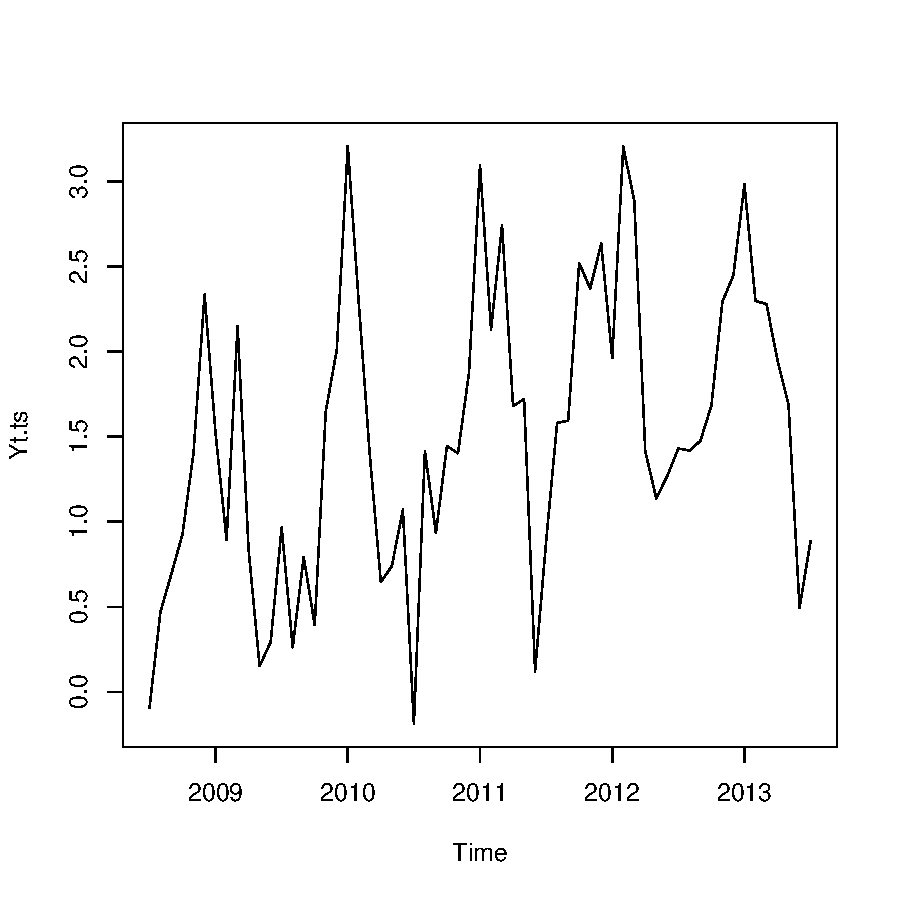
\includegraphics[height=4in, width=4in]{exercice1-graph1.pdf}
\caption{Graphique de la série $Y_t$}
\label{fig:exercice1-graph1}
\end{figure}
\item
\begin{Schunk}
\begin{Sinput}
> xtable(Zt.ts <- diff(Yt.ts,12),digits=1)
\end{Sinput}
% latex table generated in R 3.0.1 by xtable 1.7-1 package
% Wed Dec 18 23:09:09 2013
\begin{table}[ht]
\centering
\begin{tabular}{rrrrrrrrrrrrr}
  \hline
 & Jan & Feb & Mar & Apr & May & Jun & Jul & Aug & Sep & Oct & Nov & Dec \\
  \hline
2009 &  &  &  &  &  &  & 1.1 & -0.2 & 0.1 & -0.5 & 0.2 & -0.3 \\
  2010 & 1.7 & 1.4 & -0.8 & -0.2 & 0.6 & 0.8 & -1.2 & 1.2 & 0.1 & 1.1 & -0.2 & -0.1 \\
  2011 & -0.1 & -0.2 & 1.4 & 1.0 & 1.0 & -0.9 & 1.1 & 0.2 & 0.7 & 1.1 & 1.0 & 0.8 \\
  2012 & -1.1 & 1.1 & 0.1 & -0.3 & -0.6 & 1.1 & 0.5 & -0.2 & -0.1 & -0.8 & -0.1 & -0.2 \\
  2013 & 1.0 & -0.9 & -0.6 & 0.5 & 0.5 & -0.8 & -0.5 &  &  &  &  &  \\
   \hline
\end{tabular}
\end{table}\end{Schunk}

On retrouve le graphique de la série désaisonnalisée $Z_t$ à la figure \ref{fig:exercice1-graph2}.
\begin{figure}[!ht]
\centering
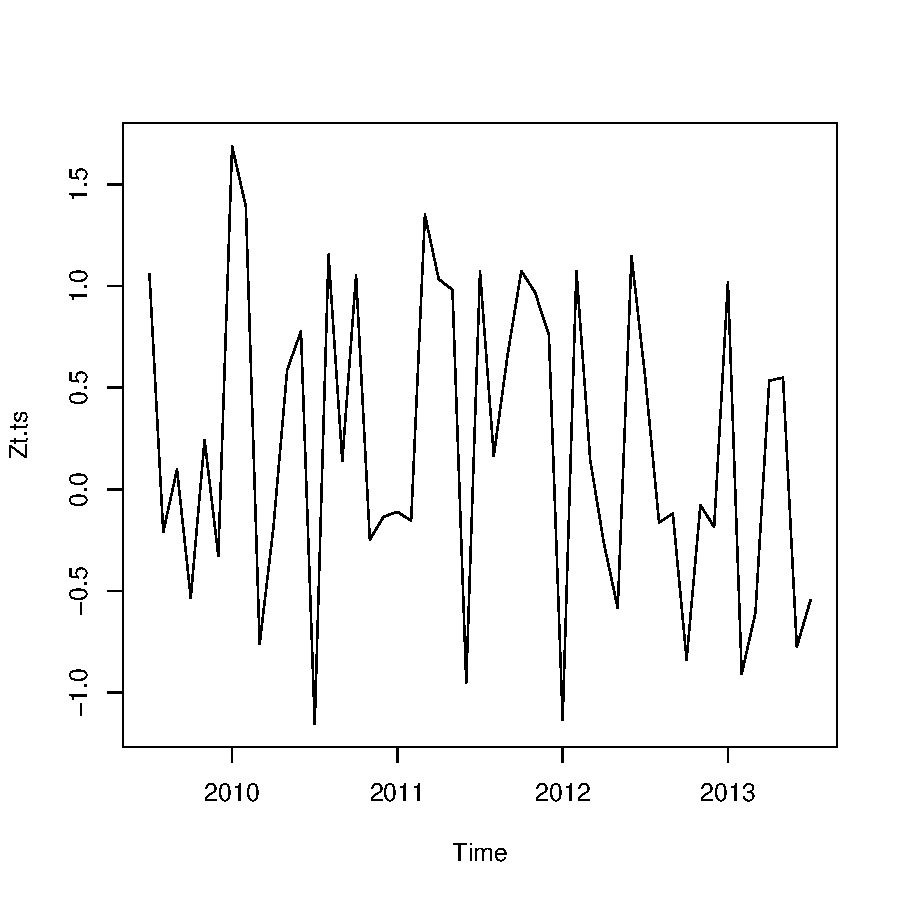
\includegraphics[height=4in, width=4in]{exercice1-graph2.pdf}
\caption{Graphique de la série désaisonnalisée $Z_t$}
\label{fig:exercice1-graph2}
\end{figure}

On élimine la composante de saisonnalité
\begin{Schunk}
\begin{Sinput}
> xtable(Yt.ts-Zt.ts,digits=1)
\end{Sinput}
% latex table generated in R 3.0.1 by xtable 1.7-1 package
% Wed Dec 18 23:09:09 2013
\begin{table}[ht]
\centering
\begin{tabular}{rrrrrrrrrrrrr}
  \hline
 & Jan & Feb & Mar & Apr & May & Jun & Jul & Aug & Sep & Oct & Nov & Dec \\
  \hline
2009 &  &  &  &  &  &  & -0.1 & 0.5 & 0.7 & 0.9 & 1.4 & 2.3 \\
  2010 & 1.5 & 0.9 & 2.2 & 0.8 & 0.2 & 0.3 & 1.0 & 0.3 & 0.8 & 0.4 & 1.6 & 2.0 \\
  2011 & 3.2 & 2.3 & 1.4 & 0.6 & 0.7 & 1.1 & -0.2 & 1.4 & 0.9 & 1.4 & 1.4 & 1.9 \\
  2012 & 3.1 & 2.1 & 2.7 & 1.7 & 1.7 & 0.1 & 0.9 & 1.6 & 1.6 & 2.5 & 2.4 & 2.6 \\
  2013 & 2.0 & 3.2 & 2.9 & 1.4 & 1.1 & 1.3 & 1.4 &  &  &  &  &  \\
   \hline
\end{tabular}
\end{table}\end{Schunk}

On retrouve le graphique de la composante de saisonnalité $Y_t-Z_t$ à la figure \ref{fig:exercice1-graph3}.
\begin{figure}[!ht]
\centering
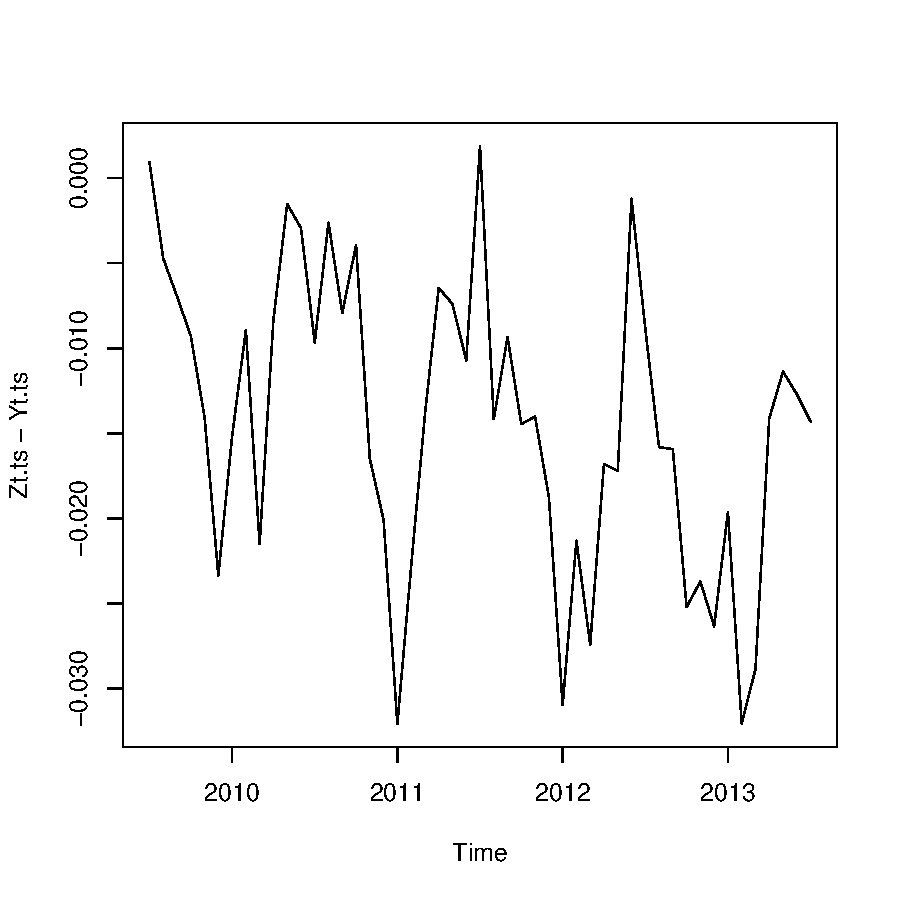
\includegraphics[height=4in, width=4in]{exercice1-graph3.pdf}
\caption{Graphique de la composante de saisonnalité $Y_t-Z_t$}
\label{fig:exercice1-graph3}
\end{figure}

\item
On élimime maintenant la tendance:

On utilise une moyenne mobile avec $q=1$. Comme la fonction \emph{SMA()} utilise les $2q+1$ données précédentes et que nous voulons une moyenne mobile centrée, nous devons utiliser l'opérateur de rétrodécalage $B()$ pour décaler la série.

\begin{Schunk}
\begin{Sinput}
> ## Simple Moving Average(q=1)
> xtable(mt1 <- lag(SMA(Zt.ts,n=3),1),digits=2)
\end{Sinput}
% latex table generated in R 3.0.1 by xtable 1.7-1 package
% Wed Dec 18 23:09:09 2013
\begin{table}[ht]
\centering
\begin{tabular}{rrrrrrrrrrrrr}
  \hline
 & Jan & Feb & Mar & Apr & May & Jun & Jul & Aug & Sep & Oct & Nov & Dec \\
  \hline
2009 &  &  &  &  &  &  &  & 0.32 & -0.22 & -0.06 & -0.21 & 0.54 \\
  2010 & 0.92 & 0.77 & 0.15 & -0.12 & 0.39 & 0.07 & 0.26 & 0.05 & 0.78 & 0.32 & 0.22 & -0.16 \\
  2011 & -0.13 & 0.36 & 0.74 & 1.12 & 0.36 & 0.37 & 0.10 & 0.63 & 0.63 & 0.90 & 0.93 & 0.20 \\
  2012 & 0.23 & 0.03 & 0.32 & -0.24 & 0.10 & 0.37 & 0.51 & 0.09 & -0.37 & -0.34 & -0.37 & 0.25 \\
  2013 & -0.02 & -0.16 & -0.33 & 0.16 & 0.10 & -0.26 &  &  &  &  &  &  \\
   \hline
\end{tabular}
\end{table}\end{Schunk}
Moyenne mobile avec $q=5$
\begin{Schunk}
\begin{Sinput}
> ## Simple Moving Average(q=5)
> xtable(mt2 <- lag(SMA(Zt.ts,n=11),5),digits=2)
\end{Sinput}
% latex table generated in R 3.0.1 by xtable 1.7-1 package
% Wed Dec 18 23:09:09 2013
\begin{table}[ht]
\centering
\begin{tabular}{rrrrrrrrrrrrr}
  \hline
 & Jan & Feb & Mar & Apr & May & Jun & Jul & Aug & Sep & Oct & Nov & Dec \\
  \hline
2009 &  &  &  &  &  &  &  &  &  &  &  & 0.28 \\
  2010 & 0.25 & 0.17 & 0.26 & 0.32 & 0.40 & 0.40 & 0.24 & 0.10 & 0.16 & 0.30 & 0.34 & 0.36 \\
  2011 & 0.37 & 0.37 & 0.37 & 0.33 & 0.45 & 0.55 & 0.63 & 0.54 & 0.52 & 0.44 & 0.32 & 0.36 \\
  2012 & 0.36 & 0.40 & 0.32 & 0.22 & 0.05 & -0.02 & 0.06 & 0.06 & -0.04 & -0.07 & 0.03 & -0.02 \\
  2013 & -0.14 & -0.18 &  &  &  &  &  &  &  &  &  &  \\
   \hline
\end{tabular}
\end{table}\end{Schunk}
Lissage exponentiel double avec $\alpha=0.75$
\begin{Schunk}
\begin{Sinput}
> ## Double Exponential Moving Average
> xtable(mt3 <- DEMA(Zt.ts,n=1,ratio=.05),digits=2)
\end{Sinput}
% latex table generated in R 3.0.1 by xtable 1.7-1 package
% Wed Dec 18 23:09:09 2013
\begin{table}[ht]
\centering
\begin{tabular}{rrrrrrrrrrrrr}
  \hline
 & Jan & Feb & Mar & Apr & May & Jun & Jul & Aug & Sep & Oct & Nov & Dec \\
  \hline
2009 &  &  &  &  &  &  & 1.06 & 0.94 & 0.85 & 0.71 & 0.66 & 0.55 \\
  2010 & 0.65 & 0.72 & 0.57 & 0.48 & 0.48 & 0.50 & 0.33 & 0.39 & 0.36 & 0.41 & 0.33 & 0.28 \\
  2011 & 0.22 & 0.17 & 0.27 & 0.33 & 0.38 & 0.24 & 0.31 & 0.29 & 0.31 & 0.38 & 0.43 & 0.45 \\
  2012 & 0.29 & 0.36 & 0.33 & 0.26 & 0.17 & 0.25 & 0.27 & 0.22 & 0.18 & 0.07 & 0.04 & 0.01 \\
  2013 & 0.09 & -0.02 & -0.09 & -0.04 & 0.00 & -0.09 & -0.14 &  &  &  &  &  \\
   \hline
\end{tabular}
\end{table}\end{Schunk}
Régression linéaire
\begin{Schunk}
\begin{Sinput}
> t <- 0:48
> (lm1 <- lm(Zt.ts~t)) ## Modèle de régression sur une variable
\end{Sinput}
\begin{Soutput}
Call:
lm(formula = Zt.ts ~ t)

Coefficients:
(Intercept)            t
   0.446924    -0.009856
\end{Soutput}
\begin{Sinput}
> coeff1 <- coefficients(lm1)
\end{Sinput}
\end{Schunk}
\begin{Schunk}
\begin{Sinput}
> xtable(mt4 <- ts(coeff1[1]+t*coeff1[2],start=c(2009,7),deltat=1/12),digits=2)
\end{Sinput}
% latex table generated in R 3.0.1 by xtable 1.7-1 package
% Wed Dec 18 23:09:09 2013
\begin{table}[ht]
\centering
\begin{tabular}{rrrrrrrrrrrrr}
  \hline
 & Jan & Feb & Mar & Apr & May & Jun & Jul & Aug & Sep & Oct & Nov & Dec \\
  \hline
2009 &  &  &  &  &  &  & 0.45 & 0.44 & 0.43 & 0.42 & 0.41 & 0.40 \\
  2010 & 0.39 & 0.38 & 0.37 & 0.36 & 0.35 & 0.34 & 0.33 & 0.32 & 0.31 & 0.30 & 0.29 & 0.28 \\
  2011 & 0.27 & 0.26 & 0.25 & 0.24 & 0.23 & 0.22 & 0.21 & 0.20 & 0.19 & 0.18 & 0.17 & 0.16 \\
  2012 & 0.15 & 0.14 & 0.13 & 0.12 & 0.11 & 0.10 & 0.09 & 0.08 & 0.07 & 0.06 & 0.05 & 0.04 \\
  2013 & 0.03 & 0.02 & 0.01 & 0.00 & -0.01 & -0.02 & -0.03 &  &  &  &  &  \\
   \hline
\end{tabular}
\end{table}\end{Schunk}
On retrouve le graphique de la tendance $m_t$ à la figure \ref{fig:exercice1-graph4}.
\begin{figure}[!ht]
\centering
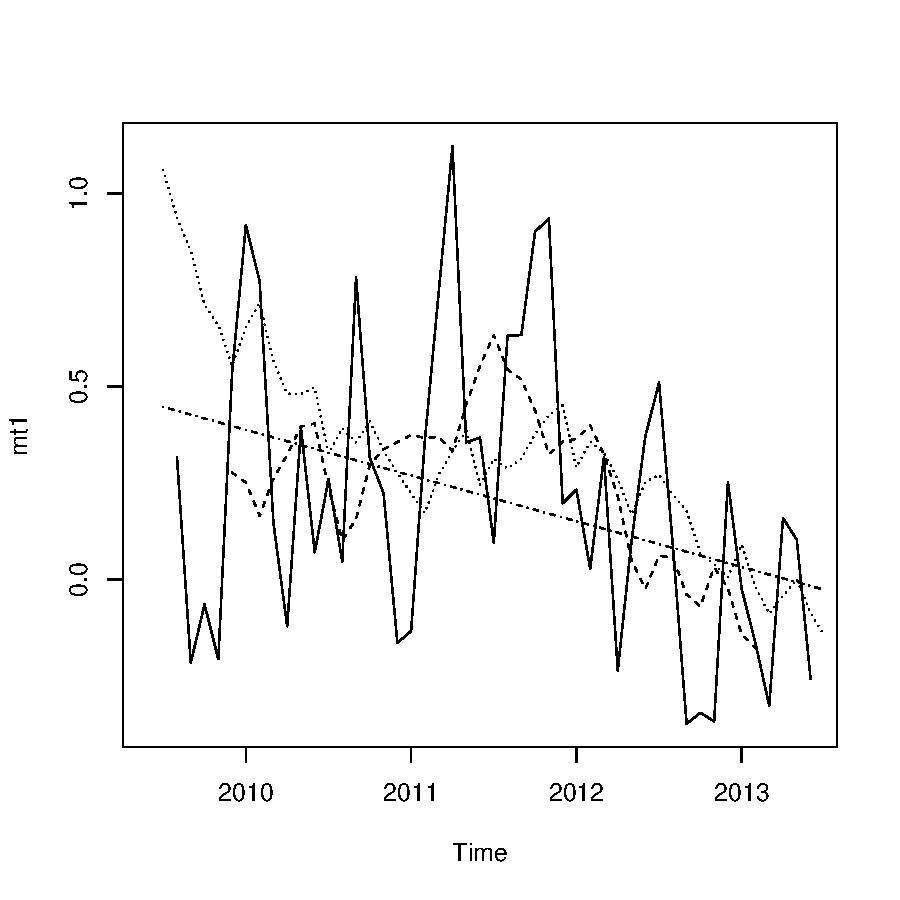
\includegraphics[height=4in, width=4in]{exercice1-graph4.pdf}
\caption{Graphique de la tendance $m_t$}
\label{fig:exercice1-graph4}
\end{figure}
\item
\begin{Schunk}
\begin{Sinput}
> projection <- coeff1[1]+53*coeff1[2]
> saisonnalite <- mean((Yt.ts-Zt.ts)[6+12*0:3])
> (taux.inf.dec.2013 <- (projection+saisonnalite))
\end{Sinput}
\begin{Soutput}
(Intercept)
   2.137743
\end{Soutput}
\end{Schunk}
Le taux d'inflation prejeté en décembre 2013 est 2.14\%
\item
\begin{Schunk}
\begin{Sinput}
> depense.dec.2008 <- 674
> depense.dec.2013 <- 674*(1+taux.inf.dec.2013/100)
\end{Sinput}
\end{Schunk}
Le montant projeté des achats de cadeaux en décembre 2013 est 688.41 \$
\end{enumerate}
\end{solution}
\begin{solution}{1.2}
On remarque d'abord que $q=2$.

On peut ensuite poser les équations suivantes:
\begin{align}
\label{eq:1}
4+3+a+b+2 &= 24\\
b+2+4+6+c &= 26\\
c+0+2+8+3 &= 19
\end{align}

En résolvant, on obtient la solution.\\

\textbf{Solution:}\\

\begin{tabular}{|l|l|l|}
\hline
\multicolumn{1}{|l|}{Mois} & \multicolumn{1}{l|}{Incendies} & \multicolumn{1}{l|}{Moyenne Mobile} \\ \hline
1 & 4 & \multicolumn{1}{l|}{-} \\ \hline
2 & 3 & \multicolumn{1}{l|}{-} \\ \hline
3 & \textbf{7} & 4,8 \\ \hline
4 & \textbf{8} & 4,8 \\ \hline
5 & 2 & 5,4 \\ \hline
6 & 4 & 5,2 \\ \hline
7 & 6 & 3,6 \\ \hline
8 & \textbf{6} & 3,6 \\ \hline
9 & 0  & 4,4 \\ \hline
10 & 2 & 3,8 \\ \hline
11 & 8 & \multicolumn{1}{l|}{-} \\ \hline
12 & 3 & \multicolumn{1}{l|}{-} \\ \hline
\end{tabular}
\end{solution}
\begin{solution}{1.3}

\begin{Schunk}
\begin{Sinput}
> rf <- 0.0175
> rB <- rf+0.02
> S0 <- 10.46
> ST <- 8.73
> K <- S0*exp(rf*84/365)
> bbry <- read.csv("blackberry.csv",header=TRUE,sep=";")
> bbry.sel <- bbry[as.POSIXlt(bbry$Date)$wday==5,][1+3:12*4,]$Close
> l.bbry.sel <- log(bbry.sel)
> (diff.l.bbry.sel <- diff(l.bbry.sel))
\end{Sinput}
\begin{Soutput}
[1]  0.288637639  0.112996047 -0.061344651 -0.103095509
[5] -0.017497594 -0.086523113  0.005008358 -0.340978628
[9] -0.090637274
\end{Soutput}
\begin{Sinput}
> (mu.diff.l.bbry.sel <- mean(diff.l.bbry.sel))
\end{Sinput}
\begin{Soutput}
[1] -0.03260386
\end{Soutput}
\begin{Sinput}
> (sigma.diff.l.bbry.sel <- sd(diff.l.bbry.sel))
\end{Sinput}
\begin{Soutput}
[1] 0.170735
\end{Soutput}
\begin{Sinput}
> (prix.arbre <- S0*(ud <- exp(3*(mu.diff.l.bbry.sel+c(1,-1)*
+                                   sigma.diff.l.bbry.sel/(2*sqrt(3))))))
\end{Sinput}
\begin{Soutput}
[1] 10.996838  8.181586
\end{Soutput}
\begin{Sinput}
> (p.rn <- (exp(rf*84/365)-ud[2])/(ud[1]-ud[2]))
\end{Sinput}
\begin{Soutput}
[1] 0.8243048
\end{Soutput}
\begin{Sinput}
> q.rn <- 1-p.rn
> (P0 <- sum(exp(-rf*84/365)*(c(p.rn,q.rn)*pmax(K-prix.arbre,0))))
\end{Sinput}
\begin{Soutput}
[1] 0.406084
\end{Soutput}
\begin{Sinput}
> (BT <- P0*exp(rB*84/365))
\end{Sinput}
\begin{Soutput}
[1] 0.4096037
\end{Soutput}
\begin{Sinput}
> (K-ST)-BT
\end{Sinput}
\begin{Soutput}
[1] 1.362608
\end{Soutput}
\end{Schunk}
La valeur du paramètre $\mu$ de rendement moyen est -0.0326.
La valeur du paramètre $\sigma$ de volatilité est 0.1707.
La valeur des prix de l'arbre binomial sont 10.9968 et 8.1816.
La valeur de la probabilité neutre au risque d'une hausse est 0.8243.
La valeur de l'option est 0.4061.
Le profit, qui correspont à la différence entre la réclamation contingente de l'option et le coût d'acquisition, est de 1.3626.
\end{solution}
\begin{solution}{1.4}
On calcule d'abord les deux séries lissées \\

\begin{tabular}{|l|r|r|}
\hline
\multicolumn{1}{|c|}{$\mathcal{A}$} & $\alpha=0,4$ & $\alpha=0,7$ \\ \hline
1,2 & 1,2000 & 1,2000 \\ \hline
1,5 & 1,3200 & 1,4100 \\ \hline
1,4 & 1,3520 & 1,4030 \\ \hline
2,1 & 1,6512 & 1,8909 \\ \hline
1,8 & 1,7107 & 1,8273 \\ \hline
1,9 & 1,7864 & 1,8782 \\ \hline
2,2 & 1,9519 & 2,1035 \\ \hline
2,4 & 2,1311 & 2,3110 \\ \hline
2,0 & 2,0787 & 2,0933 \\ \hline
1,9 & 2,0072 & 1,9580 \\ \hline
\end{tabular} \\

On évalue ensuite l'erreur quadratique pour chaque terme \\

\begin{tabular}{|l|r|r|}
\hline
\multicolumn{1}{|c|}{$\mathcal{A}$} & \multicolumn{1}{l|}{$SE(\alpha=0,4)$} & \multicolumn{1}{l|}{$SE(\alpha=0,7)$} \\ \hline
1,2 & \multicolumn{1}{l|}{} & \multicolumn{1}{l|}{} \\ \hline
1,5 & 0,0324 & 0,0081 \\ \hline
1,4 & 0,0023 & 0,0000 \\ \hline
2,1 & 0,2014 & 0,0437 \\ \hline
1,8 & 0,0080 & 0,0007 \\ \hline
1,9 & 0,0129 & 0,0005 \\ \hline
2,2 & 0,0616 & 0,0093 \\ \hline
2,4 & 0,0723 & 0,0079 \\ \hline
2,0 & 0,0062 & 0,0087 \\ \hline
1,9 & 0,0115 & 0,0034 \\ \hline
\end{tabular} \\

On obtient enfin l'erreur quadratique moyenne\\

\begin{tabular}{|l|l|l|}
\hline
& $\alpha=0,4$ & $\alpha=0,7$ \\ \hline
MSE & \multicolumn{1}{r|}{0,0454} & \multicolumn{1}{r|}{0,0092} \\ \hline
\end{tabular} \\

Les calculs effectués se trouvent dans le fichier \url{Lissage.Exponentiel.I.ods} \footnote{Ce fichier est au format OpenDocument et s'ouvre avec la plupart des suites bureautiques}.

Avec R, on obtient les résultats suivants en utilisant la fonction de lissage exponentiel \emph{EMA()}.

\begin{Schunk}
\begin{Sinput}
> A <- c(1.2, 1.5, 1.4, 2.1, 1.8, 1.9, 2.2, 2.4, 2.0, 1.9)
> n.A <- length(A)
> A.EMA.4 <- EMA(A,n=1,ratio=0.4)
> A.EMA.7 <- EMA(A,n=1,ratio=0.7)
> A.SE <- (A-cbind(A.EMA.4,A.EMA.7))^2
> cbind(A,A.EMA.4,A.EMA.7,A.SE)
\end{Sinput}
\begin{Soutput}
        A  A.EMA.4  A.EMA.7     A.EMA.4      A.EMA.7
 [1,] 1.2 1.200000 1.200000 0.000000000 0.0000000000
 [2,] 1.5 1.320000 1.410000 0.032400000 0.0081000000
 [3,] 1.4 1.352000 1.403000 0.002304000 0.0000090000
 [4,] 2.1 1.651200 1.890900 0.201421440 0.0437228100
 [5,] 1.8 1.710720 1.827270 0.007970918 0.0007436529
 [6,] 1.9 1.786432 1.878181 0.012897691 0.0004760688
 [7,] 2.2 1.951859 2.103454 0.061573857 0.0093210722
 [8,] 2.4 2.131116 2.311036 0.072298864 0.0079145417
 [9,] 2.0 2.078669 2.093311 0.006188861 0.0087069216
[10,] 1.9 2.007202 1.957993 0.011492180 0.0033632189
\end{Soutput}
\begin{Sinput}
> (A.MSE <- colMeans(A.SE)*(n.A/(n.A-1)))
\end{Sinput}
\begin{Soutput}
   A.EMA.4    A.EMA.7
0.04539420 0.00915081
\end{Soutput}
\end{Schunk}

La valeur $\alpha=0.7$ produit une erreur quadratique moyenne inférieure.
\end{solution}
\begin{solution}{1.5}
Une solution assez simple est d'utiliser le solveur intégré au logiciel tableau que vous utilisez et d'optimiser la valeur de la cellule contenant $\alpha$ avec comme critère de minimisation la cellule contenant l'erreur quadratique moyenne (MSE).

On peut aussi construire une fonction d'optimisation dans R qui réplique le comportement du chiffrier que nous avons construit dans le logiciel tableur.

\begin{Schunk}
\begin{Sinput}
> funOptAlphaDEMA <- function(alpha,data)
+ {
+   data.n <- length(data)
+   data.DEMA <- DEMA(A,n=1,ratio=alpha)
+   data.SE <- (data-data.DEMA)^2
+   data.MSE <- mean(data.SE)*data.n/(data.n-1)
+   print(c(data.MSE,alpha))
+   data.MSE
+ }
> optimize(funOptAlphaDEMA,c(0.4,0.7),A)
\end{Sinput}
\begin{Soutput}
[1] 0.006416607 0.514589803
[1] 0.003674206 0.585410197
[1] 0.002489337 0.629179607
[1] 0.001912478 0.656230590
[1] 0.001607733 0.672949017
[1] 0.001437559 0.683281573
[1] 0.001338969 0.689667444
[1] 0.00128047 0.69361413
[1] 0.001245226 0.696053315
[1] 0.001223788 0.697560814
[1] 0.001210668 0.698492500
[1] 0.001202609 0.699068314
[1] 0.001197648 0.699424186
[1] 0.001194588 0.699644128
[1] 0.0011927 0.6997801
[1] 0.001191534 0.699864069
[1] 0.001190814 0.699915990
[1] 0.00119025 0.69995669
[1] 0.00119025 0.69995669
$minimum
[1] 0.6999567

$objective
[1] 0.00119025
\end{Soutput}
\end{Schunk}

Tout comme pour le lissage exponentiel effectué à la question précédente, la valeur $\alpha=0.7$ produit une erreur quadratique moyenne inférieure.
\end{solution}
\begin{solution}{1.6}
On importe d'abord l'ensemble de données
\begin{Schunk}
\begin{Sinput}
> BoA <- ts(read.csv("BoA.csv",header=TRUE,sep="\t"))
\end{Sinput}
\end{Schunk}

\begin{enumerate}
\item
On trace ensuite le corrélogramme (figure \ref{fig:exercice1.6-graph1})
La fonction \emph{acf} nous permet d'afficher un corrélogramme
\begin{figure}[!ht]
\centering
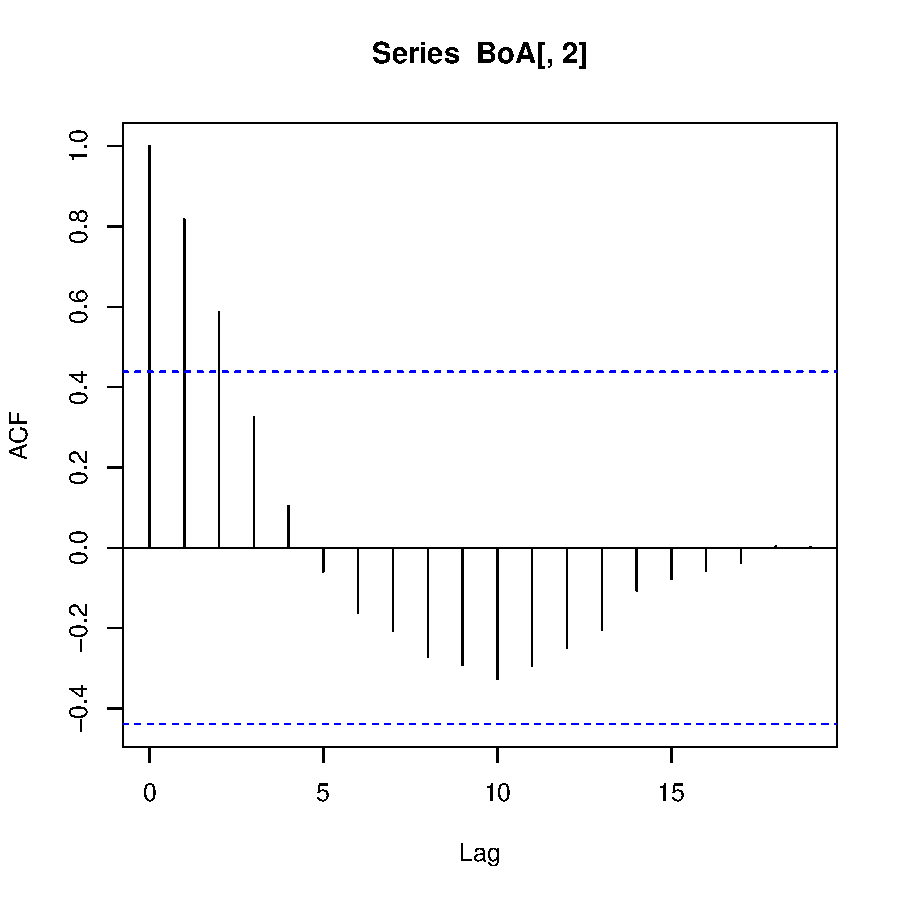
\includegraphics[height=4in, width=4in]{exercice1-6-graph1}
\caption{Corrélogramme de la série BoA}
\label{fig:exercice1.6-graph1}
\end{figure}

La fonction d'autocorrélation empirique $\hat{\rho}$ prend les valeurs
suivantes:
\begin{Schunk}
\begin{Sinput}
> (BoA.acf <- acf(BoA[,2],lag.max=19))
\end{Sinput}
\begin{Soutput}
Autocorrelations of series ‘BoA[, 2]’, by lag

     0      1      2      3      4      5      6
 1.000  0.817  0.587  0.325  0.105 -0.059 -0.161
     7      8      9     10     11     12     13
-0.207 -0.272 -0.291 -0.325 -0.293 -0.249 -0.203
    14     15     16     17     18     19
-0.106 -0.078 -0.057 -0.038  0.003  0.002
\end{Soutput}
\begin{Sinput}
> dummy <- dev.off()
\end{Sinput}
\end{Schunk}

En utilisant la méthode vue dans le cours, on construit un intervalle de
confiance au niveau $1-\alpha=0.9$ à partir de la distribution normale. La
valeur de $n$ est 20.

\begin{Schunk}
\begin{Sinput}
> (BoA.acf.IC <- round(c(1/sqrt(20)*qnorm(0.05),-1/sqrt(20)*qnorm(0.05)),4))
\end{Sinput}
\begin{Soutput}
[1] -0.3678  0.3678
\end{Soutput}
\end{Schunk}

\begin{align*}
IC &= \frac{1}{\sqrt{n}}\left[-z_{\alpha / 2},z_{\alpha / 2} \right] \\
&= \frac{1}{\sqrt{20}}\left[-z_{0.05},z_{0.05} \right] \\
&= \left[ -0.3678,0.3678 \right]
\end{align*}

\begin{Schunk}
\begin{Sinput}
> (BoA.nbacfplus <- sum(BoA.acf$acf[-1]<BoA.acf.IC[1]) +
+    sum(BoA.acf$acf[-1]>BoA.acf.IC[2]))
\end{Sinput}
\begin{Soutput}
[1] 2
\end{Soutput}
\end{Schunk}
Comme 2 valeurs sur 20, soit 10\% de celles-ci, sont à l'extérieur de
l'intervalle de confiance, alors on ne peut rejeter l'hypothèse selon laquelle la
série est stationnaire lorsqu'on se base sur le test du corrélogramme.
\item
Ici, on n'a qu'à tracer la série et compter les changements de direction
(figure \ref{fig:exercice1.6-graph2})
\begin{figure}[!ht]
\centering
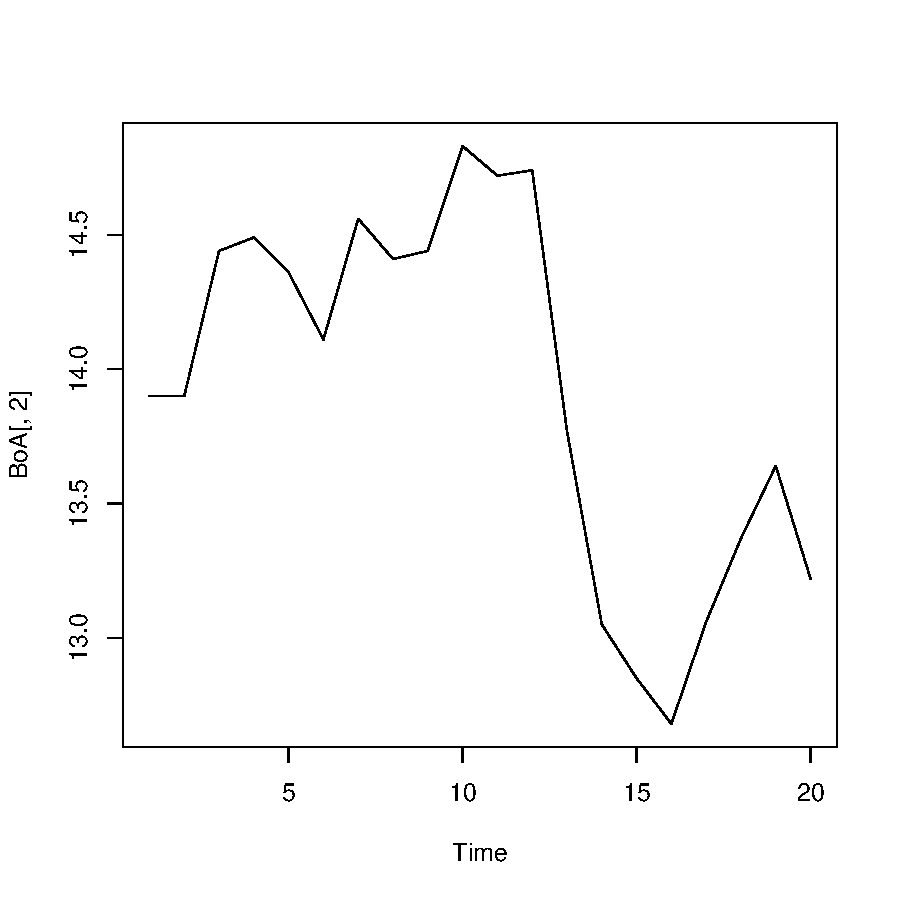
\includegraphics[height=4in, width=4in]{exercice1-6-graph2}
\caption{Corrélogramme de la série BoA}
\label{fig:exercice1.6-graph2}
\end{figure}

On en dénombre 9.

\begin{Schunk}
\begin{Sinput}
> BoA.chdir <- abs((9-(2/3)*18)/sqrt((16*20-29)/90))
> BoA.chdir > qnorm(0.95)
\end{Sinput}
\begin{Soutput}
[1] TRUE
\end{Soutput}
\end{Schunk}
On évalue la statistique de test, qui prend la valeur 1.6684. Comme cette valeur est supérieure au seuil de 1.6449, on rejette l'hypothèse de stationnarité avec le test du changement de direction.
\item
Il existe deux tests de type Portmanteau. Celui que vous avez vu en classe est le test de Box-Pierce où h commence à 1.
\begin{Schunk}
\begin{Sinput}
> Box.test(BoA[,2],lag=19,type="Box-Pierce")
\end{Sinput}
\begin{Soutput}
	Box-Pierce test

data:  BoA[, 2]
X-squared = 33.5182, df = 19, p-value = 0.02093
\end{Soutput}
\begin{Sinput}
> qchisq(0.9,19)
\end{Sinput}
\begin{Soutput}
[1] 27.20357
\end{Soutput}
\end{Schunk}

On rejette l'hypothèse de stationnarité car la valeur de $Q^{*}=33.5182$ est supérieure au quantile $\chi^2_{0.1}(19) = 27.20357$

\item
Les tests sont indépendants, différents entre eux et ne sont pas équivalents
car leurs statistiques ne suivent pas la même distribution asymptotique.

\item
\begin{Schunk}
\begin{Sinput}
> round(diff(log(BoA[,2])),4)
\end{Sinput}
\begin{Soutput}
Time Series:
Start = 2
End = 20
Frequency = 1
 [1]  0.0000  0.0381  0.0035 -0.0090 -0.0176  0.0314
 [7] -0.0104  0.0021  0.0267 -0.0074  0.0014 -0.0681
[13] -0.0537 -0.0154 -0.0133  0.0295  0.0235  0.0200
[19] -0.0313
\end{Soutput}
\end{Schunk}

\item
\begin{Schunk}
\begin{Sinput}
> (BoA.hist.var <- na.trim(apply(cbind(BoA[,2],
+                                      lag(BoA[,2],1),
+                                      lag(BoA[,2],2),
+                                      lag(BoA[,2],3),
+                                      lag(BoA[,2],4)),
+                                1,
+                                var)))
\end{Sinput}
\begin{Soutput}
 [1] 0.08642 0.06185 0.03017 0.02963 0.02753 0.06795
 [7] 0.03257 0.03617 0.18785 0.61597 0.79813 0.71857
[13] 0.17257 0.06697 0.15075 0.12818
\end{Soutput}
\begin{Sinput}
> Box.test(BoA.hist.var,lag=15,type="Box-Pierce")
\end{Sinput}
\begin{Soutput}
	Box-Pierce test

data:  BoA.hist.var
X-squared = 13.7076, df = 15, p-value = 0.5478
\end{Soutput}
\begin{Sinput}
> qchisq(0.9,15)
\end{Sinput}
\begin{Soutput}
[1] 22.30713
\end{Soutput}
\end{Schunk}

On remarque que la série des volatilités historiques avec $q=2$ est stationnaire bien que la volatilité ne soit pas constante.
\end{enumerate}
\end{solution}
\begin{solution}{1.7}
La variance du $t^e$ terme est équivalente à la somme de la variance des $t$ premiers termes d'erreurs. La différence entre les variances des $5^e$ terme et du $7^e$ terme est donc égale à la somme:
\begin{align*}
\label{eq:2}
V\left[\epsilon_6\right]+V\left[\epsilon_7\right] &= 0.1(6^2+7^2) \\
& = 8.5
\end{align*}
\end{solution}

\section*{Chapitre \ref{chap:modeles-classiques}}
\addcontentsline{toc}{section}{Chapitre \protect\ref{chap:modeles-classiques}}

\begin{solution}{2.1}
  On obtient les racines de l'équation caractéristique en utilisant la formule quadratique habituelle

\begin{align*}
\frac{\phi_1\pm\sqrt{\phi_1^2+4\phi_2}}{-2\phi_2}
\end{align*}

On considère les inverses des deux racines, $A_1$ et $A_2$.

\begin{align*}
A_1 &= \frac{2\phi_2}{-\phi_1-\sqrt{\phi_1^2+4\phi_2}} \\
&= \frac{2\phi_2}{-\phi_1-\sqrt{\phi_1^2+4\phi_2}} \left[\frac{-\phi_1+\sqrt{\phi_1^2+4\phi_2}}{-\phi_1+\sqrt{\phi_1^2+4\phi_2}} \right] \\
&= \frac{2\phi_2(-\phi_1+\sqrt{\phi_1^2+4\phi_2})}{\phi_1^2-(\phi_1^2+4\phi_2)}\\
&= \frac{\phi_1-\sqrt{\phi_1^2+4\phi_2}}{2}\\
A_2 &= \frac{\phi_1+\sqrt{\phi_1^2+4\phi_2}}{2}
\end{align*}

Il y a 2 situations possibles: soit les racines sont réelles ($\phi_1^2+4\phi_2>0$) ou elles sont complexes ($\phi_1^2+4\phi_2<0$).
\begin{itemize}
\item \textbf{Racines réelles:}
Comme les racines doivent être plus grandes que 1, alors nécessairement leurs inverses $|A_1|<1$ et $|A_2|<1$. Nous avons donc:
\begin{align*}
-1 &< \frac{\phi_1-\sqrt{\phi_1^2+4\phi_2}}{2} <  \frac{\phi_1+\sqrt{\phi_1^2+4\phi_2}}{2} < 1 \\
\Leftrightarrow -2 &< \phi_1-\sqrt{\phi_1^2+4\phi_2} < \phi_1+\sqrt{\phi_1^2+4\phi_2} < 2
\end{align*}
En observant la première inégalité, on a:
\begin{align*}
-2 < \phi_1-\sqrt{\phi_1^2+4\phi_2}
&\Leftrightarrow \sqrt{\phi_1^2+4\phi_2}<\phi_1+2 \\
&\Leftrightarrow \phi_1^2+4\phi_2 < \phi_1^2+4\phi_1+4 \\
&\Leftrightarrow \phi_2 < \phi_1 + 1 \\
&\Leftrightarrow \phi_2 - \phi_1 < 1
\end{align*}
Ce qui correspond à la seconde condition. En considérant la seconde inégalité, on obtient, de la même façon, la première inégalité:
\begin{align*}
\phi_1+\sqrt{\phi_1^2+4\phi_2} &< 2 \\
&\Leftrightarrow \phi_1 + \phi_2 < 1
\end{align*}
Ces deux conditions réunies avec un discriminant positif forment la région de stationnarité pour des racines réelles.

\item \textbf{Racines complexes:}
On considère la situation où $\phi_1^2+4\phi_2<0$. Ici, on aura des conjugués complexes et $|A_1| = |A_2| <1$ seulement si $|A_1|^2<1$.
\begin{align*}
|A_1|^2 &=\frac{\phi_1^2+(-\phi_1^2-4\phi_2}{4}=-\phi^2 \\
&\Leftrightarrow \phi_2>-1 \\
&\Leftrightarrow |\phi_2|<1
\end{align*}
Ce résultat réuni avec un discriminant négatif forment la région de stationnarité pour des racines complexes.
\end{itemize}
\end{solution}
\begin{solution}{2.2}
\begin{enumerate}

\item On obtient ce résultat par récurrence. Par exemple, pour $k=2$, on a :

\begin{align*}
(1-B)^2 (a_0+a_1t+a_2t^2) &= (1-B) ((a_0+a_1t+a_2t^2)\\ &\quad- (a_0+a_1(t-1)+a_2(t-1)^2)) \\
&= (1-B) (a_1+a_2(2t+1)) \\
&= (a_1+a_2(2t+1)) - (a_1+a_2(2(t-1)+1)) \\
&= 2a_2
\end{align*}

En général, on obtient:

\begin{align*}
(1-B)^k (a_0+a_1t+a_2t^2+\ldots+a_kt^k) &= (1-B)^{k-1} ((a_0+a_1t+a_2t^2+\ldots+a_kt^k)\\ &\quad- (a_0+a_1(t-1)+a_2(t-1)^2+\ldots+a_k(t-1)^k)) \\
&= (1-B)^{k-1} (a_1 + 2a_2t+\ldots+a_k(t^k-(t-1)^k))
\end{align*}

On remarque qu'à chaque itération, le premier terme de la série disparait. Ainsi, après $k$ itérations, il ne restera que le terme en $a_k$ avec son coefficient, qui correspont à $k!$. On obtient ainsi la solution générale.

\item Une série est dite stationnaire lorsque chaque terme est un terme d'erreur dont la distribution est constante au fil du temps. Ainsi, la distribution de la différence de deux termes consécutifs de la série sera aussi constante au fil du temps. Par exemple:
\begin{align*}
\epsilon_t \sim N(0,\sigma^2)  \\
\epsilon_t - \epsilon_{t-1} \sim N(0,2\sigma^2) \\
\end{align*}

\end{enumerate}
\end{solution}
\begin{solution}{2.3}
  \begin{enumerate}
\item Un processus AR(1) est défini par $y_t = \phi_1y_{t-1} + \epsilon_t$. En développant le terme $y_{t-1}$, on obtient $y_t = \phi_1^2y_{t-2}+\phi_1\epsilon_{t-1}+\epsilon_t$. De manière récursive, on obtient $y_t = \phi_1^{t}\epsilon_0 + \phi_1^{t-1}\epsilon_1 + \ldots + \phi_1\epsilon_{t-1} + \epsilon_t$. ainsi, en faisant tendre $t\to\infty$, on obtient une représentation MA($\infty$).

\item Un processus MA(1) est défini par $y_t = \epsilon_t - \theta_1\epsilon_{t-1}$. On cherche à substituer le terme $\epsilon_{t-1}$. On développe le terme précédent de la série: $y_{t-1} = \epsilon_{t-1} - \theta_1\epsilon_{t-2}$ et on substitue dans la première expression pour obtenir $y_t = \epsilon_t - \theta_1y_{t-1} - \theta_1^2\epsilon_{t-2}$. De manière récursive, on obtient $y_t = -\theta_1^ty_0-\theta_1^{t-1}y_1-\ldots-\theta_1y_{t-1}+\epsilon_{t}$. Lorsque $t\to\infty$, on obtient une représentation AR($\infty$).
\end{enumerate}
\end{solution}
\begin{solution}{2.4}
  On utilise la formule $y_t = \phi_1y_{t-1} + \epsilon_t$.

\begin{center}
\begin{tabular}{|r|r|r|}
\hline
\multicolumn{1}{|l|}{} & \multicolumn{ 2}{c|}{$\phi$} \\ \hline
\multicolumn{1}{|l|}{$N(0,1)$} & -0,5 & 0,5 \\ \hline
-1,21 & -1,2100 & -1,2100 \\ \hline
0,28 & 0,8850 & -0,3250 \\ \hline
1,08 & 0,6375 & 0,9175 \\ \hline
-2,35 & -2,6688 & -1,8913 \\ \hline
0,43 & 1,7644 & -0,5156 \\ \hline
0,51 & -0,3722 & 0,2522 \\ \hline
-0,57 & -0,3839 & -0,4439 \\ \hline
-0,55 & -0,3580 & -0,7720 \\ \hline
-0,56 & -0,3810 & -0,9460 \\ \hline
-0,89 & -0,6995 & -1,3630 \\ \hline
\end{tabular}
\end{center}

Les séries avec une corrélation négative ont tendance à aller dans la direction contraire des termes précédents alors que celles avec une corrélation positive ont tendance à aller dans la même direction que les termes précédents.

Le tableur \url{constructionserieAR.ods} contient les calculs effectués.
\end{solution}
\begin{solution}{2.5}
    Il suffit de calculer la fonction d'autorégression pour chaque processus MA(2).
Ensuite, on peut évaluer la fonction d'autocorrélation et comparer le résultat obtenu.

\begin{enumerate}
\item Premier processus avec:
\begin{align*}
\theta_1 = \theta_2 = \frac{1}{4}
\end{align*}
Fonction d'autocovariance
\begin{align*}
\phi_0^{(1)} &= V[Y_t] \\
&= V[e_t]+\frac{1}{16}V[e_{t-1}]+\frac{1}{16}V[e_{t-2}] \\
&= (1+\frac{1}{8})\theta^2_e \\
&= \frac{9}{8} \sigma^2_e \\
\end{align*}
\begin{align*}
\phi_1^{(1)} &= Cov(Y_t,Y_{t-1}) \\
&= Cov(e_t - \frac{1}{4}e_{t-1} - \frac{1}{4}e_{t-2}, e_{t-1} - \frac{1}{4}e_{t-2} - \frac{1}{4}e_{t-3} )\\
&= Cov(-\frac{1}{4}e_{t-1},e_{t-1}) + Cov(-\frac{1}{4}e_{t-2},-\frac{1}{4}e_{t-2}) \\
&= (-\frac{1}{4}+(-\frac{1}{4})(-\frac{1}{4})) \sigma^2_e \\
&= -\frac{3}{16} \sigma^2_e \\
\end{align*}
\begin{align*}
\phi_2^{(1)} &= Cov(Y_t,Y_{t-2}) \\
&= Cov(e_t - \frac{1}{4}e_{t-1} - \frac{1}{4}e_{t-2}, e_{t-2} - \frac{1}{4}e_{t-3} - \frac{1}{4}e_{t-4} )\\
&= Cov(-\frac{1}{4}e_{t-2},e_{t-2}) \\
&= -\frac{1}{4} \sigma^2_e \\
\end{align*}
\begin{align*}
\phi_k^{(1)} &= 0, \qquad \forall k \geq 3
\end{align*}
Fonction d'autocorrélation
\begin{align*}
\rho_1^{(1)} &= \frac{\phi_1^{(1)}}{\phi_0^{(1)}} \\
&= \frac{\frac{-3}{16}\sigma^2_e}{\frac{9}{8}\sigma^2_e} \\
&= \frac{-1}{6} \\
\end{align*}
\begin{align*}
\rho_2^{(1)} &= \frac{\phi_2^{(1)}}{\phi_0^{(1)}} \\
&= \frac{\frac{-1}{4}\sigma^2_e}{\frac{9}{8}\sigma^2_e} \\
&= \frac{-2}{9} \\
\end{align*}
\item Second processus avec:
\begin{align*}
\theta_1 = -1 \quad \theta_2 = 4
\end{align*}
Fonction d'autocovariance
\begin{align*}
\phi_0^{(2)} &= V[Y_t] \\
&= V[e_t]+V[e_{t-1}]+16V[e_{t-2}] \\
&= 18 \sigma^2_e
\end{align*}
\begin{align*}
\phi_1^{(2)} &= Cov(Y_t,Y_{t-1}) \\
&= Cov(e_t + e_{t-1} - 4e_{t-2}, e_{t-1} + e_{t-2} - 4e_{t-3}) \\
&= Cov(e_{t-1},e_{t-1}) + Cov(-4e_{t-2},e_{t-2}) \\
&= (1 + (-1)(4))\sigma^2_e \\
&= -3\sigma^2_e \\
\end{align*}
\begin{align*}
\phi_2^{(2)} &= Cov(Y_t,Y_{t-2}) \\
&= Cov(e_t + e_{t-1} - 4e_{t-2}, e_{t-2} + e_{t-3} - 4e_{t-4} )\\
&= Cov(- 4e_{t-2},e_{t-2}) \\
&= -4\sigma^2_e \\
\end{align*}
Fonction d'autocorrélation
\begin{align*}
\rho_1^{(2)} &= \frac{\phi_1^{(2)}}{\phi_0^{(2)}} \\
&= \frac{-3\sigma^2_e}{18\sigma^2_e} \\
&= \frac{-1}{6} \\
\end{align*}
\begin{align*}
\rho_2^{(2)} &= \frac{\phi_2^{(2)}}{\phi_0^{(2)}} \\
&= \frac{-4\sigma^2_e}{18\sigma^2_e} \\
&= \frac{-2}{9} \\
\end{align*}
\end{enumerate}

On remarque clairement que $\rho_1^{(1)} = \rho_1^{(2)}$ et $\rho_2^{(1)} = \rho_2^{(2)}$.
La fonction d'autocovariance vaut toujours 1 pour $\rho_1$ et vaut 0 ailleurs.
  
\end{solution}
\begin{solution}{2.6}
  \begin{enumerate}
\item
Les deux équations de Yule-Walker pour le modèle AR(2) sont les suivantes:
\begin{align*}
\rho_1 = \phi_1 + \rho_1 \phi_2 \\
\rho_2 = \rho_1\phi_1 + \phi_2
\end{align*}

En utilisant l'estimateur de la fonction d'autocovariance $\hat{\rho}$, on obtient alors:

\begin{align*}
\hat{\phi_1} = \frac{\hat{\rho_1}(1-\hat{\rho_2})}{1-\hat{\rho_1}^2} \\
\hat{\phi_2} = \frac{\hat{\rho_2} - \hat{\rho_1}^2}{1-\hat{\rho_1}^2}
\end{align*}


\item

\begin{Schunk}
\begin{Sinput}
> set.seed(123)
> (serie <- arima.sim(n = 10, list(ar = c(0.5,-0.25))))
\end{Sinput}
\begin{Soutput}
Time Series:
Start = 1
End = 10
Frequency = 1
 [1]  1.1617660  0.6981185  0.1693004 -0.6457205
 [5]  1.4217278  1.3701445 -1.6369769 -0.4596686
 [9] -0.2933815 -1.0995973
\end{Soutput}
\begin{Sinput}
> acf.serie <- acf(serie,type="correlation",plot=FALSE)$acf[2:3]
> phi1 <- acf.serie[1]*(1-acf.serie[2]) / (1-acf.serie[1]^2)
> phi2 <- (acf.serie[2] - acf.serie[1]^2) / (1-acf.serie[1]^2)
\end{Sinput}
\end{Schunk}

On obtient $\hat{\rho_1} = 0.07455$ et $\hat{\rho_2} = -0.28041$.
Ce qui nous donne les paramètres du modèle AR(2) suivants:
$\hat{\phi_1} = 0.09599$ et
$\hat{\phi_2} = -0.28757$.
\end{enumerate}
\end{solution}
\begin{solution}{2.7}
  \begin{enumerate}
\item
  On représente le processus ARMA(2,1) sous la forme suivante:
  \begin{align*}
    y_t = \mu + \phi_1 y_{t-1} + \phi_2 y_{t-2} + \epsilon_t - \theta\epsilon_{t-1}
  \end{align*}

  En utilisant l'opérateur de rétrodécalage $B$, on peut exprimer cette équation sous la forme suivante:
  \begin{align*}
    (1-\theta B)\epsilon_t = y_t - \mu - \phi_1 y_{t-1} - \phi_2 y_{t-2}
  \end{align*}

  On divise ensuite de chaque côté par $(1-\theta B)$, pour obtenir:
  \begin{align*}
    \epsilon_t = \frac{1}{(1-\theta B)} \left(y_t - \mu - \phi_1 y_{t-1} - \phi_2 y_{t-2}\right)
  \end{align*}

  L'hypothèse de stationnarité nous permet de poser que $| \theta | < 1$, ce qui nous permet d'utiliser la série géométrique définie comme suit:
  \begin{align*}
    \frac{1}{1-\theta B} = \sum_{i=0}^{\infty} \theta^i B^i
  \end{align*}

  On obtient donc que
  \begin{align*}
    \epsilon_t = \sum_{i=0}^{\infty} \theta^i B^i \left(y_t - \mu - \phi_1 y_{t-1} - \phi_2 y_{t-2}\right)
  \end{align*}

  En appliquant l'opérateur de rétrodécalage à la parenthèse, on obtient la solution:
  \begin{align*}
    \epsilon_t = \sum_{i=0}^{\infty} \theta^i \left(y_{t-i} - \mu - \phi_1 y_{t-i-1} - \phi_2 y_{t-i-2} \right)
  \end{align*}

\item

  On exprime l'équation précédente en fonction de $y_t$:
  \begin{align*}
    y_t &= \phi_1 y_{t-1} + \phi_2 y_{t-2} - \sum_{i=1}^{\infty} \theta^i \left(y_{t-i} - \phi_1 y_{t-i-1} - \phi_2 y_{t-i-2} \right) + \epsilon_t + \frac{\mu}{1-\theta} \\
    &= \phi_1 y_{t-1} + \phi_2 y_{t-2} - \left[\theta\left(y_{t-1}-\phi_1 y_{t-2} - \phi_2 y_{t-3} \right) + \sum_{i=2}^{\infty} \theta^i \left(y_{t-i} - \phi_1 y_{t-i-1} - \phi_2 y_{t-i-2} \right)\right] + \epsilon_t + \frac{\mu}{1-\theta}  \\
    &= (\phi_1 - \theta) y_{t-1} - \sum_{i=2}^{\infty} \left(\theta_i+\phi_1\theta^{i-1} - \phi_2\theta_{i-2}\right) y_{t-i} + \epsilon_t + \frac{\mu}{1-\theta}
  \end{align*}
  Ce qui correspont à la forme autorégressive AR($\infty$) suivante:
  \begin{align*}
    y_t = c + \sum_{i=1}^{\infty} \pi_i y_{t-i} + \epsilon_t
  \end{align*}
  Avec les paramètres
  \begin{align*}
    c &= \frac{\mu}{1-\theta} \\
    \pi_1 &= (\phi_1 - \theta) \\
    \pi_i &= -\left(\theta_i+\phi_1\theta^{i-1} - \phi_2\theta_{i-2}\right),\quad i=2,3,\ldots
  \end{align*}
\end{enumerate}
\end{solution}
\begin{solution}{2.8}
  \begin{enumerate}
\item C'est un modèle AR(2) de paramètres $\phi_1=1.5$ et $\phi_2=-0.5$.
\item L'équation caractéristique prend la forme suivante:
  \begin{align*}
    y_t - 1.5 y_{t-1} + 0.5y_{t-2} = 0
  \end{align*}

  On pose la solution générale $y_t=A\alpha^t$:
  \begin{align*}
    A\alpha^t - 1.5 A\alpha^{t-1} + 0.5A\alpha^{t-2} = 0
  \end{align*}

  On divise ensuite par $A\alpha^{t-2}$:
  \begin{align*}
    0 &= \alpha^2 - 1.5 \alpha + 0.5\\
    \alpha &= \frac{1.5 \pm \sqrt{1.5^2-4*1*0.5}}{2} \\
    &= \left\{0.5 ; 1 \right\}
  \end{align*}

\item
  \begin{align*}
    1 - 1.5B + 0.5B^2 &= 0 \\
    (1-B)(1-0.5B) &= 0
  \end{align*}
  Ce qui nous donne:
  \begin{align*}
    B &= \left\{ 1;2 \right\} \\
    B^{-1} &= \left\{ 1;0.5 \right\}
  \end{align*}

\item Nous n'avons pas la stationnarité, car $\alpha$ n'est pas à l'intérieur du cercle unité

\item
  \begin{align*}
    y_2 &= 1.5 y_1 - 0.5y_0 + \epsilon_2 \\
    y_3 &= 1.5 y_2 - 0.5y_1 + \epsilon_3 \\
    &= \epsilon_3 + 1.5 \epsilon_2 + 1.75y_1 - 0.75 y_0 \\
    y_4 &= 1.5 y_3 - 0.5y_2 + \epsilon_4 \\
    &= \epsilon_4 + 1.5 \epsilon_3 + 1.75 \epsilon_2 + 1.875 y_1 - 0.875 y_0
  \end{align*}

  On peut observer un motif répétifif, que l'on représente sous la forme
  \begin{align*}
    y_t &= \sum_{i=0}^{t-2} \alpha_i\epsilon_{t-i} + \alpha_{t-1}y_1 + \alpha_t y_0 \\
  \end{align*}
  où
  \begin{align*}
    \alpha_0 &= 1\\
    \alpha_1 &= 1.5\\
    \alpha_t &= 1-\alpha_{t-1}
    \alpha_i &= 1.5 \alpha_{i-1} - 0.5 \alpha_{i-2}
  \end{align*}
\item
  \begin{align*}
    y_s &= \sum_{i=0}^{s-2} \alpha_i\epsilon_{s-i} + \alpha_{s-1}y_1 + \alpha_s y_0 \\
    y_{t+s} &= \sum_{i=0}^{s-2} \alpha_i\epsilon_{t+s-i} + \alpha_{s-1}y_{t+1} + \alpha_s y_t \\
    E_{t+1}\left[y_{t+s}\right] &= \alpha_{s-1} y_{t+1} + \alpha_s y_t
  \end{align*}

\item
  \begin{align*}
    E\left[y_t\right] &= \alpha_{t-1} y_1 + \alpha_t y_0 \\
    E\left[y_{t+1}\right] &= \alpha_{t} y_1 + \alpha_{t+1} y_0 \\
    Var\left[y_t\right] &= \left[1+\alpha_1^2 + \alpha_2^2 + \ldots + \alpha_{t-2}^2\right]\sigma^2 \\
    Var\left[y_{t+1}\right] &= Var\left[y_t\right] + \alpha_{t-1}^2 \sigma^2 \\
    Cov\left[y_{t},y_{t+1}\right] &= \left[\alpha_0\alpha_1 + \alpha_1\alpha_2 + \ldots + \alpha_{t-3}\alpha_{t-2}\right] \sigma^2
  \end{align*}
\item
  \begin{align*}
    \alpha_{t} y_1 + \alpha_{t+1} y_0 \pm 1.96 * \sigma \sqrt{1+\alpha_1^2 + \alpha_2^2 + \ldots + \alpha_{t-2}^2+\alpha_{t-1}^2}
  \end{align*}
\end{enumerate}
\end{solution}
\begin{solution}{2.9}
  \begin{enumerate}
\item
  \begin{align*}
    Var[X_t] &= Var[Y_t] + Var[Z_t] \\
    &= (1+\alpha^2)\sigma^2_{V} + \sigma^2_{\delta} \\
    E[X_t,X_{t-1}] &= E[(v_t+\delta_t+\alpha v_{t-1})(v_{t-1}+\delta_{t-1}+\alpha v_{t-2})] \\
    &= \alpha \sigma^2_{V} \\
    E[X_t,X_{t-k}] &= 0, \quad\forall k \neq \{ 0,1 \} \\
    &\Rightarrow \gamma_0,\gamma_1 \neq 0; \gamma_k=0 \forall k \neq \{ 0,1 \} \\
  \end{align*}
  Par conséquent, il s'agit d'un modèle MA(1).
\item
  \begin{align*}
    \gamma_0 &= (1+\theta_1^2) \sigma^2_{\epsilon} = (1+\alpha^2)\sigma^2_{V} + \sigma^2_{\delta} \\
    \gamma_1 &= \theta\sigma^2_{\epsilon} = \alpha\sigma^2_{V}
  \end{align*}
  On résous ce système d'équations numériquement:


\begin{Schunk}
\begin{Sinput}
> fun1 <- function(par,alpha,sV,sdelta)
+ {
+   sqrt(((1+alpha^2)*sV+sdelta-(1+par[1]^2)*par[2])^2
+        +(alpha*sV-par[1]*par[2])^2)
+ }
> paramoptimaux1 <- round(optim(c(0.4,0.04),fun1,,0.5,0.04,0.01)$par,5)
\end{Sinput}
\end{Schunk}

On a donc que $\theta$ = 0.38197 et $\sigma^2_{\epsilon}$ = 0.05236
  On obtient le meme résultat en utilisant un logiciel de calcul symbolique comme Maxima.
  \end{enumerate}
\end{solution}
\begin{solution}{2.10}
    \begin{align*}
  E_t[x_{t+2}] &= \phi^2 x_t = 0.4^2*1.5 = 0.24 \\
  V_t[x_{t+2}] &= (1+\phi^2)\sigma^2_{\epsilon} = (1+0.4^2)*0.25 = 0.29
\end{align*}

Intervalle de confiance:

\begin{align*}
  IC &= E_t[x_{t+2}] \pm \Phi^{-1}(0.975)\sqrt{V_t[x_{t+2}]} \\
  &= 0.4^2*1.5 \pm 1.96 \sqrt{(1+0.4^2)*0.25} \\
  &= [-0.815492;1.295492]
\end{align*}
  
\end{solution}

\section*{Chapitre \ref{chap:modeles-volatilite}}
\addcontentsline{toc}{section}{Chapitre \protect\ref{chap:modeles-volatilite}}

\begin{solution}{3.1}
  On identifie d'abord la moyenne conditionnelle de $y_t$:
\begin{align}
E_{t-1}[y_t] &= E_{t-1}[a_0 + a_1 y_{t-1} + \epsilon_t] \\
&= a_0 + a_1 y_{t-1}
\end{align}
La variance conditionnelle peut alors s'obtenir en utilisant la définition habituelle:
\begin{align*}
V_{t-1}[y_t | y_{t-1}, y_{t-2}, \ldots] &= E_{t-1}[y_t - E_{t-1}[y_t]]^{2} \\
&= E_{t-1}[(a_0 + a_1 y_{t-1} + \epsilon_t)-(a_0 + a_1 y_{t-1})]^{2} \\
&= E_{t-1}[\epsilon_t]^{2} \\
&= E_{t-1}[\alpha_0 + \alpha_1\epsilon_{t-1}^2 + \alpha_2\epsilon_{t-2}^2] \\
&= \alpha_0 + \alpha_1\epsilon_{t-1}^2 + \alpha_2\epsilon_{t-2}^2
\end{align*}

La variance inconditionnelle s'obtient en trouvant la solution particulière pour $y_t$:
\begin{align*}
•y_t &= a_0 + a_1 y_{t-1} + \epsilon_t \\
&= (1+a_1)a_0 + a_1^2 y_{t-2} + a_1 \epsilon_{t-1} + \epsilon_t \\
&= \cdots \\
&= (a+a_1+a_2+a_3+\ldots)a_0 + \epsilon_t + a_1\epsilon_{t-1} + a_2\epsilon_{t-2} + \ldots \\
&= \frac{a_0}{1-a_1} + \sum_{i=0}^{\infty} a_1^{i}\epsilon_{t-i}
\end{align*}

On évalue la variance de cette dernière expression:
\begin{align*}
•Var[y_t] &= Var[\sum_{i=0}^{\infty} a_1^{i}\epsilon_{t-i}] \\
&= \sum_{i=0}^{\infty} a_1^{2i} Var[\epsilon_{t-i}] \\
&= \frac{\sigma^2}{1-a_1^2}
\end{align*}

À partir de la définition, on a que:
\begin{align*}
E[\epsilon_t^2] &= \alpha_0 + \alpha_1 E_[\epsilon_{t-1}^2] + \alpha_2 E[\epsilon_{t-2}^2].
\end{align*}

Comme la variance inconditionnelle de $\epsilon_t$ est identique à celle de $\epsilon_{t-1}$ et $\epsilon_{t-2}$, on peut affirmer que:
\begin{align*}
E[\epsilon_t^2] &= \frac{\alpha_0}{1-\alpha_1-\alpha_2} \\
&= \sigma^2.
\end{align*}

On obtient donc que la variance inconditionnelle de $y_t$ est
\begin{align*}
•Var[y_t] &= \frac{\alpha_0}{(1-\alpha_1-\alpha_2)(1-a_1^2)}.
\end{align*}
\end{solution}


%%% Local Variables:
%%% mode: latex
%%% TeX-master: "exercices_series_chrono"
%%% End:

\pagestyle{empty}

\includegraphics[height=7mm,keepaspectratio=true]{by-sa}\\%
Cette création est mise à disposition selon le contrat
\href{http://creativecommons.org/licenses/by-sa/2.5/ca/deed.fr}{%
  Paternité-Partage à l'identique 2.5 Canada} de Creative Commons
disponible à l'adresse \\
http://creativecommons.org/licenses/by-sa/2.5/ca/deed.fr \\

En vertu de ce contrat, vous êtes libre de :

\begin{itemize}
\item \textbf{partager} --- reproduire, distribuer et communiquer
  l'{\oe}uvre;
\item \textbf{remixer} --- adapter l'{\oe}uvre;
\item utiliser cette {\oe}uvre à des fins commerciales.
\end{itemize}

Selon les conditions suivantes:\\

  \begin{tabularx}{\linewidth}{@{}lX@{}}
    \raisebox{-9mm}[0mm][13mm]{%
      
\includegraphics[height=11mm,keepaspectratio=true]{by}} &
    \textbf{Attribution} --- Vous devez attribuer l'{\oe}uvre de la
    manière indiquée par l'auteur de l'{\oe}uvre ou le titulaire des
    droits (mais pas d'une manière qui suggérerait qu'ils vous
    soutiennent ou
    approuvent votre utilisation de l'{\oe}uvre). \\
    \raisebox{-9mm}{
\includegraphics[height=11mm,keepaspectratio=true]{sa}}
    & \textbf{Partage à l'identique} --- Si vous modifiez, transformez
    ou adaptez cette {\oe}uvre, vous n'avez le droit de distribuer
    votre création que sous une licence identique ou similaire à
    celle-ci.
  \end{tabularx}

%%% Local Variables: 
%%% mode: latex
%%% TeX-master: t
%%% End: 

\cleardoublepage
\cleartoverso

\pagestyle{empty}
\bandeverso

\end{document}

%%% Local Variables:
%%% mode: latex
%%% TeX-master: t
%%% End:
